\documentclass[a4paper,fleqn]{cas-sc}



\usepackage{amsmath,amssymb}
\usepackage{booktabs}
\usepackage{graphicx}
\usepackage{siunitx}
\sisetup{round-mode=places, round-precision=3}
\usepackage[authoryear,round]{natbib}
\setcitestyle{aysep={, },citesep={; }}
\usepackage[all]{hypcap}
\usepackage{cleveref}
\crefname{appendix}{appendix}{appendices}
\Crefname{appendix}{Appendix}{Appendices}
\crefname{algocf}{algorithm}{algorithms}
\Crefname{algocf}{Algorithm}{Algorithms}

\usepackage[ruled,vlined,linesnumbered]{algorithm2e}
%\SetAlgoSkip{0pt}   % put once in preamble
\SetAlgoNoEnd
% Change only these lines to point the note at another rendered report.
\newcommand{\reportroot}{.}
\newcommand{\datasetlabel}{HundredPatches/norm}
\newcommand{\distanceboxplot}{\reportroot/images/distance_profiles_box_whisker/linear/distance_iqr_medians_rainy_multi_k3_box_whisker.png}
\newcommand{\nonrainydistanceboxplot}{\reportroot/images/distance_profiles_box_whisker/linear/distance_iqr_medians_nonrainy_multi_k3_box_whisker.png}
\newcommand{\idwconfusionplot}{\reportroot/images/confusion_maps/IDW_confusion_map.png}
\newcommand{\ildwconfusionplot}{\reportroot/images/confusion_maps/ILDW_confusion_map.png}
\newcommand{\nonlinearconfusionplot}{\reportroot/images/confusion_maps/Nonlinear_Optimizer_confusion_map.png}
\newcommand{\patchgeometryplot}{\reportroot/images/patch_overview/patch_dimensions_scatter.png}
\newcommand{\patcheuropeoverview}{\reportroot/images/patch_overview/hundredpatches_europe_overview_basemap.png}
\newcommand{\patchmetricboxplot}{\reportroot/images/summaries/patch_map_metrics_boxplots_readable_corr.png}
\newcommand{\linkhistplot}{\reportroot/images/patch_overview/link_count_histogram.png}
\newcommand{\largestpatchbinsplot}{\reportroot/images/largest_patch_distance_bins/largest_patch_distance_bins_k3.png}
\newcommand{\contextroot}{\reportroot/images/rain_patch_explorer_maps}
\newcommand{\contextvone}{\reportroot/images/rain_patch_explorer_maps/v1}
\newcommand{\contextvtwo}{\reportroot/images/rain_patch_explorer_maps/v2}
\newcommand{\contextscreenshotorigone}{\contextvone/202301280900_patch000_map.png}
\newcommand{\contextscreenshotorigtwo}{\contextvone/202301310900_patch000_map.png}
\newcommand{\contextscreenshotone}{\contextvtwo/RAD_OPERA_HOURLY_RAINFALL_ACCUMULATION_202301282100_patch000.png}
\newcommand{\contextscreenshottwo}{\contextvtwo/RAD_OPERA_HOURLY_RAINFALL_ACCUMULATION_202301310200_patch000.png}
\newcommand{\contextscreenshotthree}{\contextvone/202301311600_patch000_map.png}
\newcommand{\combinedcaseorigone}{\reportroot/images/patch_error_maps/combined/RAD_OPERA_HOURLY_RAINFALL_ACCUMULATION_202301280900_patch000.png}
\newcommand{\gtconvexcaseone}{\reportroot/images/case_studies/new_pattern_one/RAD_OPERA_HOURLY_RAINFALL_ACCUMULATION_202301280900_patch000.png}
\newcommand{\jgtcaseone}{\reportroot/images/j_behavior/gt_vs_convex_pattern_one/case1-gt-iterations.png}
\newcommand{\jconvexcaseone}{\reportroot/images/j_behavior/gt_vs_convex_pattern_one/case1-convex-iterations.png}
\newcommand{\gtconvexcasetwo}{\reportroot/images/case_studies/new_pattern_one/RAD_OPERA_HOURLY_RAINFALL_ACCUMULATION_202301310900_patch000.png}
\newcommand{\jgtcasetwo}{\reportroot/images/j_behavior/gt_vs_convex_pattern_one/case2-gt-iterations.png}
\newcommand{\jconvexcasetwo}{\reportroot/images/j_behavior/gt_vs_convex_pattern_one/case2-convex-iterations.png}
\newcommand{\combinedcaseorigtwo}{\reportroot/images/patch_error_maps/combined/RAD_OPERA_HOURLY_RAINFALL_ACCUMULATION_202301310900_patch000.png}
\newcommand{\combinedcaseone}{\reportroot/images/patch_error_maps/combined/RAD_OPERA_HOURLY_RAINFALL_ACCUMULATION_202301282100_patch000.png}
\newcommand{\combinedcasetwo}{\reportroot/images/patch_error_maps/combined/RAD_OPERA_HOURLY_RAINFALL_ACCUMULATION_202301310200_patch000.png}
\newcommand{\combinedcasethree}{\reportroot/images/patch_error_maps/combined/RAD_OPERA_HOURLY_RAINFALL_ACCUMULATION_202301311600_patch000.png}
\newcommand{\idwcaseorigone}{\reportroot/images/patch_error_maps/IDW/RAD_OPERA_HOURLY_RAINFALL_ACCUMULATION_202301280900_patch000_rainy.png}
\newcommand{\ildwcaseorigone}{\reportroot/images/patch_error_maps/ILDW/RAD_OPERA_HOURLY_RAINFALL_ACCUMULATION_202301280900_patch000_rainy.png}
\newcommand{\optcaseorigone}{\reportroot/images/patch_error_maps/OPT_NORM_ILDW_MULT_ILDW_INIT/RAD_OPERA_HOURLY_RAINFALL_ACCUMULATION_202301280900_patch000_rainy.png}
\newcommand{\idwcaseorigtwo}{\reportroot/images/patch_error_maps/IDW/RAD_OPERA_HOURLY_RAINFALL_ACCUMULATION_202301310900_patch000_rainy.png}
\newcommand{\ildwcaseorigtwo}{\reportroot/images/patch_error_maps/ILDW/RAD_OPERA_HOURLY_RAINFALL_ACCUMULATION_202301310900_patch000_rainy.png}
\newcommand{\optcaseorigtwo}{\reportroot/images/patch_error_maps/OPT_NORM_ILDW_MULT_ILDW_INIT/RAD_OPERA_HOURLY_RAINFALL_ACCUMULATION_202301310900_patch000_rainy.png}
\newcommand{\idwcaseone}{\reportroot/images/patch_error_maps/IDW/RAD_OPERA_HOURLY_RAINFALL_ACCUMULATION_202301282100_patch000_rainy.png}
\newcommand{\ildwcaseone}{\reportroot/images/patch_error_maps/ILDW/RAD_OPERA_HOURLY_RAINFALL_ACCUMULATION_202301282100_patch000_rainy.png}
\newcommand{\optcaseone}{\reportroot/images/patch_error_maps/OPT_NORM_ILDW_MULT_ILDW_INIT/RAD_OPERA_HOURLY_RAINFALL_ACCUMULATION_202301282100_patch000_rainy.png}
\newcommand{\idwcasetwo}{\reportroot/images/patch_error_maps/IDW/RAD_OPERA_HOURLY_RAINFALL_ACCUMULATION_202301310200_patch000_rainy.png}
\newcommand{\ildwcasetwo}{\reportroot/images/patch_error_maps/ILDW/RAD_OPERA_HOURLY_RAINFALL_ACCUMULATION_202301310200_patch000_rainy.png}
\newcommand{\optcasetwo}{\reportroot/images/patch_error_maps/OPT_NORM_ILDW_MULT_ILDW_INIT/RAD_OPERA_HOURLY_RAINFALL_ACCUMULATION_202301310200_patch000_rainy.png}
\newcommand{\idwcasethree}{\reportroot/images/patch_error_maps/IDW/RAD_OPERA_HOURLY_RAINFALL_ACCUMULATION_202301311600_patch000_rainy.png}
\newcommand{\ildwcasethree}{\reportroot/images/patch_error_maps/ILDW/RAD_OPERA_HOURLY_RAINFALL_ACCUMULATION_202301311600_patch000_rainy.png}
\newcommand{\optcasethree}{\reportroot/images/patch_error_maps/OPT_NORM_ILDW_MULT_ILDW_INIT/RAD_OPERA_HOURLY_RAINFALL_ACCUMULATION_202301311600_patch000_rainy.png}
\newcommand{\jcaseorigone}{\reportroot/images/j_behavior/opt_norm_ildw_mult_ildw_init/RAD_OPERA_HOURLY_RAINFALL_ACCUMULATION_202301280900_patch000.png}
\newcommand{\jcaseorigtwo}{\reportroot/images/j_behavior/opt_norm_ildw_mult_ildw_init/RAD_OPERA_HOURLY_RAINFALL_ACCUMULATION_202301310900_patch000.png}
\newcommand{\jcaseone}{\reportroot/images/j_behavior/opt_norm_ildw_mult_ildw_init/RAD_OPERA_HOURLY_RAINFALL_ACCUMULATION_202301282100_patch000.png}
\newcommand{\jcasetwo}{\reportroot/images/j_behavior/opt_norm_ildw_mult_ildw_init/RAD_OPERA_HOURLY_RAINFALL_ACCUMULATION_202301310200_patch000.png}
\newcommand{\jcasethree}{\reportroot/images/j_behavior/opt_norm_ildw_mult_ildw_init/RAD_OPERA_HOURLY_RAINFALL_ACCUMULATION_202301311600_patch000.png}


\newcommand{\notebox}[3]{%
  \begingroup
  \setlength{\fboxsep}{2pt}%
  \fcolorbox{#1}{#2}{\textsf{\footnotesize #3}}%
  \endgroup
}

\DeclareRobustCommand{\editnote}[1]{%
  \texorpdfstring{%
    \nobreak\hfill
    \mbox{\notebox{red!50!black}{red!10}{#1}}%
  }{}%
}

\DeclareRobustCommand{\inlinenote}[1]{%
  \mbox{\notebox{red!50!black}{red!10}{#1}}%
}

\newcommand{\editsection}[2]{\section[#1]{#1\editnote{#2}}}
\newcommand{\editsubsection}[2]{\subsection[#1]{#1\editnote{#2}}}


%algs
\DeclareRobustCommand{\IDW}{\textsc{idw}}
\DeclareRobustCommand{\ILDW}{\textsc{ildw}}
\DeclareRobustCommand{\solverILDW}{\textsc{solver(ildw)}}
\DeclareRobustCommand{\solverGT}{\textsc{solver(gt)}}
\DeclareRobustCommand{\solverConvex}{\textsc{convex solver}}
\DeclareRobustCommand{\solverHomotopy}{\textsc{homotopy solver}}
\DeclareRobustCommand{\ConvexSolver}{\solverConvex}
\DeclareRobustCommand{\Homotopy}{\solverHomotopy}
\DeclareRobustCommand{\LBFGSB}{\textsc{lbfgsb}}
\DeclareRobustCommand{\OPTILDW}{\solverILDW}

% Column labels and compact numeric notation.
\newcommand{\RMSE}{RMSE}
\newcommand{\Bias}{Bias}
\newcommand{\Pearson}{Pearson $r$}
\newcommand{\meanPixels}{mean pixels}
\newcommand{\pmv}[2]{#1\,$\pm$\,#2}


\begin{document}
\let\WriteBookmarks\relax
\def\floatpagepagefraction{1}
\def\textpagefraction{.001}

\shorttitle{Precipitation Estimation from Commercial Microwave Links}
\shortauthors{G. Even et al.}

\title[mode=title]{Discrete Learning Algorithms for Precipitation Estimation from Commercial Microwave Links}

\author[mpi]{Guy Even}
\ead{guyeven@mpi-inf.mpg.de}

\author[mpi]{Andreas Karrenbauer}
\ead{andreas.karrenbauer@mpi-inf.mpg.de}


\author[mpi]{Rex Lei}
\ead{rexlei@mpi-inf.mpg.de}

\author[tau]{Jonatan Ostrometzky}
\ead{jonatano@tauex.tau.ac.il}

\author[cologne]{Christian Sohler}
\ead{sohler@cs.uni-koeln.de}

\author[mpi]{Iv\'an Soto}
\ead{ivanalisv@gmail.com}

\affiliation[mpi]{organization={MPI for Informatics},
  city={Saarbr\"ucken},
  country={Germany}}

\affiliation[tau]{organization={School of Electrical Engineering, Tel-Aviv University},
  city={Tel Aviv},
  country={Israel}}

\affiliation[cologne]{organization={University of Cologne},
  city={Cologne},
  country={Germany}}

\begin{abstract}
  Commercial microwave links (CMLs) are part of the infrastructure of wireless networks. Their measured attenuations have been studied as an opportunistic source for monitoring spatiotemporal rainfall and other atmospheric phenomena. CML attenuation measurements can enhance the spatiotemporal accuracy and resolution of existing weather monitoring instruments. In addition, they serve as stand-alone weather monitoring devices in places where dedicated weather monitoring devices are scarce or do not exist.

  Current techniques for 2D rainfall map reconstruction usually reduce CML measurements to virtual rain gauges, namely point measurements, and rely on interpolation techniques such as inverse distance weighting or Kriging. While effective in many scenarios, these methods are suboptimal because they do not address the modeling error introduced when a path-integrated attenuation measurement is replaced by a single-point rain-intensity value.

  In this study, we revisit the rainfall map reconstruction problem from CML signal attenuation measurements with a principled optimization approach. We formulate the problem of partial-to-complete field reconstruction as a physics-informed optimization problem. The reconstructed rainfall field is quantized and represented by pixel rainfall variables whose values are constrained to agree with the observed CML signal attenuations. The resulting solution minimizes a weighted sum of attenuation errors along the links, spatial differences between neighboring pixels, and the total rainfall over the map.

  To evaluate our approach, we create a benchmark of hundreds of rainfall maps and CML configurations. Rainfall maps are extracted from EURADCLIM by identifying rain events over patches of approximately $50 \times 50$ km$^2$ across diverse terrain types and precipitation patterns. CMLs are overlaid using a publicly available Netherlands dataset, and attenuations are computed using the ITU-R P.838 model.

  We then solve the inverse problem to reconstruct rainfall maps from attenuations and compare the results with inverse distance weighting. Overall, this study reframes rainfall reconstruction from opportunistic sensing networks as a well-posed inverse problem with an explicit objective function. The framework also provides interpretability benefits compared to purely data-driven approaches.
\end{abstract}

\begin{highlights}
  \item Rainfall reconstruction from CMLs is formulated as an explicit inverse optimization problem.
  \item A benchmark is built from EURADCLIM rain maps and synthetic link attenuations.
  \item The formulation preserves path geometry instead of collapsing links to point measurements.
\end{highlights}

\begin{keywords}
  Commercial microwave links \sep Rainfall estimation \sep Inverse problems \sep Optimization \sep Remote sensing
\end{keywords}

\maketitle

\section{Introduction\editnote{GE:need complete rewrite}}
\section{Introduction}

Accurate rainfall estimation is a major tool used for accurate hydrology studies, weather prediction, flood forecasting, and urban drainage management. Reliable information on the spatial and temporal structure of precipitation is particularly important in urban and densely populated environments, where short-duration convective events may produce strong local gradients and rapid hydrological response. Conventional weather monitoring tools, primarily rain gauges and weather radars, provide valuable information but also have well-known limitations. Rain gauges offer direct point measurements, and are considered very accurate when properly installed, but their spatial density is often insufficient for resolving localized rainfall variability. Weather radars provide wide-area coverage, yet their estimates are not at ground level, and are prone to many uncertainties such as scattering, blockages, unaccounted vertical variability of rainfall, and limited near-ground representativeness.

Commercial microwave links (CMLs) offer a complementary source of rainfall information. These links are widely deployed as part of cellular telecommunication backhaul networks and continuously transmit electromagnetic signals between fixed antennas in a line-of-sight installments, nowadays at frequencies of 10 GHz to 90 GHz. During rainfall, raindrops affect the microwave radiation, causing measurable attenuation of the received signal. Since the frequencies range of operational links are sensitive to rain-induced attenuation \cite{ITU,gunn1954microwave,olsen1978rain}, the same infrastructure for communication was shown to also serve as an opportunistic environmental sensing network \cite{RemkoCountry2,chwala2019cml,fencl2015commercial}. As the CMLs are already deployed at large scale, often form dense networks in urban and suburban areas (especially in recent times, where dedicated CMLs networks for smart-city management are being deployed \cite{ostrometzky2024opportunistic,janco2022rain}, and are gaining attention as part of the integrated sensing and communication (ISAC) paradigm \cite{han2023potential}), they can provide near-ground measurements integrated along their paths, which span between tens of meters to several kilometers. Note that CMLs can be used in combination with satellite microwave links (SML) to further enhance their capabilities \cite{nebuloni2025review}. %Not sure we need the last sentence, it is for us to be able to shove a citation...

The physical basis for CML rainfall sensing is based on the attenuation of the signal that is caused by precipitation \cite{gunn1954microwave, olsen1978rain}, and is described by the ITU-R power-law relation\editnote{AK: We should cite the standard here, but which one is the right one?} between rain rate and specific attenuation. Given the frequency and polarization of a link, the rain-induced attenuation accumulated along the link can be modeled as the path integral of the specific attenuation over the rainfall field. Thus, unlike a rain gauge, which measures rainfall at a point, a CML provides a path-integrated measurement. This distinction is fundamental. A single link does not directly observe the rainfall value at one location; rather, it constrains the average attenuation, and hence the rainfall intensity, along its propagation path. Consequently, rainfall reconstruction from CMLs is an inverse problem: the objective is to estimate a spatial rainfall field from a collection of line-integral-like measurements.

Many practical CML-based reconstruction methods simplify this inverse problem by first converting each link measurement into a single representative rain-rate value, often interpreted as a virtual rain gauge located at the link midpoint or at an assumed other point along the link path. Standard spatial interpolation techniques can then be applied to these virtual point observations. This approach is simple, computationally efficient, and often useful in practice. However, it also discards part of the geometric information contained in the link measurement. In particular, the fact that the attenuation is accumulated along an extended path is replaced by a point approximation. This simplification may introduce modeling errors, especially in heterogeneous rainfall fields or in regions where the geometry and density of the link network strongly influence the information available for reconstruction \cite{gat2019comparative,Leijnse2008}. %TODO: Add some references about paths

A more faithful treatment of CML data should account for the coupling between the unknown rainfall field and the measured attenuation along each link path. This coupling depends on the link geometry, length, frequency, polarization, and the spatial distribution of rain along the path. Reconstruction methods that explicitly incorporate this structure have the potential to use the available information more effectively, but they also lead to more challenging estimation problems. In particular, because the attenuation--rain-rate relation is nonlinear, the corresponding inverse problem may be formulated as a constrained nonconvex optimization problem over the rainfall field.

Evaluating such reconstruction methods is difficult in real operational settings because the true rainfall field is generally unknown. Real CML measurements also include additional effects that complicate the analysis, such as wet-antenna attenuation, baseline drift, quantization, hardware-dependent sampling, and measurement noise. While these effects are essential in operational systems, they make it difficult to isolate the intrinsic performance of the reconstruction algorithm itself. A controlled benchmark, in which the ground-truth rainfall field is known and the corresponding CML attenuations are generated through a forward physical model, provides a useful way to study this core inverse problem.

In this paper, we introduce such a benchmark framework. Starting from hourly EURADCLIM rainfall maps, we construct synthetic but physically grounded rain-event patches and generate corresponding noise-free CML attenuation measurements using the ITU-R forward model. This creates a controlled evaluation setting in which different reconstruction algorithms can be compared directly against the known rainfall field. By removing confounding measurement artifacts while preserving realistic spatial rainfall patterns, the proposed benchmark isolates the reconstruction problem and enables systematic analysis of the role of link geometry, interpolation assumptions, and optimization-based estimation.

We use this framework to compare standard inverse-distance weighting (IDW), a link-aware extension tailored to CML measurements, and a nonconvex optimization formulation that directly couples the estimated rainfall field to the measured attenuations.\editnote{AK: We should cite something for the other two methods} In addition, we analyze reconstruction quality as a function of distance from the available links, thereby quantifying how the spatial arrangement of the CML network affects estimation accuracy.

\subsection{Contributions}
\begin{enumerate}
  \item Introduction of a methodology for generating rain-event benchmarks for evaluation of rainfall estimation based on noise-free CML attenuation.
  \item Creation of a benchmark (750 patches).
  \item Introduction of a new algorithm ILDW - version of IDW tailored for CML's.
  \item Introduction of rain-rate estimation as a nonconvex constrained optimization problem. Improve coupling between the estimation and measured attenuation.
  \item Systematic evaluation of IDW, ILDW, and nonconvex optimization algorithms.
  \item Evidence of quality of estimates as a function of distance from links.

\end{enumerate}
%%%%%%%%%%%%%%%%%%%%%%%%%%%%%%%%%%%%%%%%%%%%%%%%%%%%%
\section{Background and Related Work}
\subsection{ITU-R Forward Model: Rain-Induced Attenuation }

During a rain event, the signal along a commercial microwave link experiences attenuation because raindrops absorb and scatter electromagnetic energy.
We use Recommendation ITU-R P.838-3 for converting rain-rate into specific attenuation~\citep{ITU}. The ITU-R model relates the rain rate $R$ (in \si{\milli\meter\per\hour})
to the \emph{specific attenuation} $\gamma_R$ (in \si{\deci\bel\per\kilo\meter}) through the power law
\begin{equation}\label{eq:ITU}
  \gamma_R = \kappa R^{\alpha},
\end{equation}
where the coefficients $\kappa$ and $\alpha$ depend on the link frequency and polarization \citep{ITU}. See Table~\ref{tab:itu_coeffs} for the coefficient values and resulting attenuation for horizontal polarization and rain rates of $1$--$8$ \si{\milli\meter\per\hour}.

The total rain-induced attenuation is the integral of $\gamma_R$ along the link. Thus, longer links accumulate more attenuation, and links operating at different frequencies or polarizations respond differently to the same rainfall field.
For a horizontal terrestrial link of length $L$ with uniform rain rate $R$ along the path, the total rain-induced attenuation is therefore $A=\gamma_R \cdot L$.
If the rain-rate field is discretized into pixels, the total rain-induced attenuation is the sum of the attenuations over the segments obtained by intersecting the link with the pixels it traverses.


%%%
\begin{table}[t]
  \centering
  \caption{ITU-R P.838-3 coefficients for horizontal polarization and resulting specific attenuation $\gamma_R$ for selected rain rates (\si{\milli\meter\per\hour}).}
  \label{tab:itu_coeffs}
  \begin{tabular}{
      S[table-format=2.0, round-mode=places, round-precision=0]
      S[table-format=1.5]
      S[table-format=1.3]
      S[table-format=1.3]
      S[table-format=1.3]
      S[table-format=1.3]
      S[table-format=1.3]
    }
    \hline
    \multicolumn{1}{c}{$f$}                            &
    \multicolumn{1}{c}{$\kappa_H$}                     &
    \multicolumn{1}{c}{$\alpha_H$}                     &
    \multicolumn{1}{c}{$\gamma_R(R=1)$}                &
    \multicolumn{1}{c}{$\gamma_R(R=2)$}                &
    \multicolumn{1}{c}{$\gamma_R(R=4)$}                &
    \multicolumn{1}{c}{$\gamma_R(R=8)$}                                                                               \\
    \multicolumn{1}{c}{(\si{\giga\hertz})}             &
    \multicolumn{1}{c}{}                               &
    \multicolumn{1}{c}{}                               &
    \multicolumn{1}{c}{(\si{\decibel\per\kilo\meter})} &
    \multicolumn{1}{c}{(\si{\decibel\per\kilo\meter})} &
    \multicolumn{1}{c}{(\si{\decibel\per\kilo\meter})} &
    \multicolumn{1}{c}{(\si{\decibel\per\kilo\meter})}                                                                \\
    \hline
    10                                                 & 0.01217 & 1.257  & 0.01217 & 0.0290861 & 0.069515 & 0.166140 \\
    15                                                 & 0.04481 & 1.1233 & 0.04481 & 0.0976162 & 0.212652 & 0.463251 \\
    20                                                 & 0.09164 & 1.0568 & 0.09164 & 0.1906398 & 0.396590 & 0.825032 \\
    25                                                 & 0.1571  & 0.9991 & 0.1571  & 0.3140041 & 0.627616 & 1.254450 \\
    30                                                 & 0.2403  & 0.9485 & 0.2403  & 0.4637466 & 0.894968 & 1.727168 \\
    40                                                 & 0.4431  & 0.8673 & 0.4431  & 0.8083232 & 1.474580 & 2.689996 \\
    \hline
  \end{tabular}
\end{table}
%%%

%%%%%%%%%%%%%%%%%%%%%%%%%%%%%%%%%%%%%%%%%%%%%%%%%%%%%
\section{Benchmark Construction\editnote{GE:stable}}
In this section, we describe how we constructed our benchmark of rain-event patches combined with CML rain-attenuation.  The resulting benchmark instances combine realistically derived rainfall maps with real-world link configurations, from which noise-free rain-induced attenuation measurements are generated for every link.
\subsection{Data Source}
We extract rain events from the European climatological gauge-adjusted radar precipitation dataset EURADCLIM \citep{overeem2023euradclim}. EURADCLIM is derived from OPERA European radar composites and provides hourly precipitation fields at 2 \si{\kilo\meter} spatial resolution over a large fraction of Europe. The dataset are distributed in HDF5 format according to the OPERA Data Information Model (ODIM) convention \citep{odimh5}. File-level access and documentation are provided through the KNMI data platform \citep{knmi_euradclim_project}.

\subsection{Automatic Extraction of Rain Events}
To obtain benchmark instances of manageable and comparable size, hourly maps are processed independently and rain events are extracted as spatial patches. We threshold a locally averaged rainfall field, compute connected components of the thresholded pixels, and keep only components whose bounding-box side lengths fall within a prescribed size. In this way, each retained event corresponds to a rain patch. \editnote{AK: mention size here}

%The extraction procedure is:
%\begin{enumerate}
%\item Compute a local mean version of the rainfall field using a $4 \times 4$ uniform averaging window.
%\item Keep pixels whose smoothed rainfall exceeds a threshold of 3.0 mm.
%\item Partition the retained pixels into connected components.
%\item Keep only those components whose bounding boxes have side lengths between 50 km and 95 km.
%\end{enumerate}


\subsection{Refinement and Smoothing}
We refine and smooth each rain patch derived from EURADCLIM rainfall maps by subdividing each pixel into $16 \times 16$ subpixels (each $125 \times 125$ m$^2$), followed by Gaussian smoothing with $\sigma = 1$ in subpixel units.
The resulting rain patches are treated as the ground-truth rainfall field.

\subsection{CML Dataset}
CML metadata (including link locations, lengths, and frequencies) are obtained from the publicly available 4TU dataset~\citep{overeem2016cml} (we assumed horizontal polarization for all links). For each rainfall patch, the set of links is cropped to the patch extent and overlaid on the rainfall field. The ITU-R rain-attenuation model is then applied along each link path to compute the corresponding attenuation values.

\begin{table}[!htbp]
  \centering
  \begin{tabular}{lrrrrr}
    \toprule
    Patch size (km) & \# links & 1-multiplicity & 2-multiplicity \\
    \midrule
    $50 \times 50$  & 939      & 99             & 420            \\
    $62 \times 60$  & 1254     & 128            & 563            \\
    $72 \times 70$  & 1507     & 157            & 675            \\
    \bottomrule
  \end{tabular}
  \caption{Representative link multiplicities for three patch dimensions.
    The multiplicity of a link is defined as the number of frequencies assigned to it.
    The second column reports the total number of link–frequency pairs.
    In the data set, link multiplicities were either 1 or 2, with approximately $10\%$ of links having multiplicity 1.
  }
  \label{tbl:4TU link multiplicities}
\end{table}

\section{Benchmark Statistics}
In this section, we summarize key properties of the benchmark patches and their associated link geometry. We describe the geographic distribution and size range of the selected rain events, illustrate representative patch instances, summarize link statistics and topology, and report how rainy and dry pixels are distributed with respect to distance from the third-closest link.
%%%%%%%%%
%%%%%
%%
\paragraph{Patches.}
\begin{description}

  \item[Time.] The rain patches were extracted from hourly EURADCLIM maps between 18 and 31 January 2023.

  \item[Geographic distribution.] See \Cref{fig:patches_europe_overview} for a depiction of the geographic locations of the $100$ rain patches.

        \begin{figure}[!htbp]
          \centering
          \includegraphics[width=0.5\textwidth]{\patcheuropeoverview}
          \caption{Geographic locations of the $100$ benchmark patches.}
          \label{fig:patches_europe_overview}
        \end{figure}

  \item[Patch sizes.]
        A scatter diagram of patch side lengths is depicted in \Cref{fig:patch scatter}. The smallest patch is $50 \times 50$ \si{\kilo\meter} and the largest is $88 \times 88$ \si{\kilo\meter}.


        \begin{figure}[!htbp]
          \centering
          \includegraphics[width=0.82\textwidth]{\patchgeometryplot}
          \caption{Patch width versus patch height for the 100 benchmark patches, with one dot per patch.  Across patches, the mean patch area is 269,491 pixels with SD of 76,755 pixels (pixels are squares with side length $125$ m).}
          \label{fig:patch scatter}
        \end{figure}

  \item[Sample patches.] Sample rain-events from the benchmark are depicted in \Cref{fig:case_gt_convex_202301280900,fig:case_gt_convex_202301310900} together with their geographic location.
\end{description}
%%%%%%%%%
%%%%%
%%
\paragraph{Links.}
A depiction of the links in the largest $88\times 88$ \si{\kilo\meter} patch appears in \Cref{fig:largest_patch_distance_bins}.
The pixels in this figure are binned according to their distance to the third-closest link. For a pixel $p$, let $d_3(p)$ denote the distance from the pixel center to the third-closest link. Equivalently, $d_3(p)$ is the smallest radius such that a disk centered at $p$ intersects at least three links.

\Cref{tab:largest_patch_distributions} provides data about the distribution of link lengths, frequencies and endpoint degrees in this patch (the degree of an endpoint is number of links incident to this endpoint). See \Cref{tbl:4TU link multiplicities} for the number of links and their multiplicities for typical patch sizes (multiplicity $2$ means a link operating in two frequencies).


\begin{figure}[!b]
  \centering
  \includegraphics[width=0.88\textwidth]{\largestpatchbinsplot}
  \caption{$d_3$-bin map for the largest evaluated patch in the benchmark. Each pixel is colored according to its $d_3$ bin, and the complete link geometry is overlaid in white.}

  \label{fig:largest_patch_distance_bins}
\end{figure}

\begin{table}[!htbp]
  \centering
  \begin{minipage}[t]{0.31\textwidth}
    \centering
    \scriptsize
    \begin{tabular}{lrr}
      \toprule
      Length bin (km) & Count & \%   \\
      \midrule
      $[0,1)$         & 330   & 17.4 \\
      $[1,2)$         & 515   & 27.2 \\
      $[2,4)$         & 546   & 28.8 \\
      $[4,8)$         & 387   & 20.4 \\
      $[8,16)$        & 109   & 5.8  \\
      $[16,24]$       & 7     & 0.4  \\
      \bottomrule
    \end{tabular}
  \end{minipage}
  \hfill
  \begin{minipage}[t]{0.31\textwidth}
    \centering
    \scriptsize
    \begin{tabular}{lrr}
      \toprule
      Frequency bin (GHz) & Count & \%   \\
      \midrule
      $[10,15)$           & 20    & 1.1  \\
      $[15,20)$           & 67    & 3.5  \\
      $[20,25)$           & 79    & 4.2  \\
      $[25,30)$           & 257   & 13.6 \\
      $[30,35)$           & 84    & 4.4  \\
      $[35,40)$           & 1306  & 69.0 \\
      $[40,60]$           & 81    & 4.3  \\
      \bottomrule
    \end{tabular}
  \end{minipage}
  \hfill
  \begin{minipage}[t]{0.31\textwidth}
    \centering
    \scriptsize
    \begin{tabular}{lrr}
      \toprule
      Endpoint-degree bin & Count & \%   \\
      \midrule
      $1$                 & 168   & 15.0 \\
      $2$                 & 560   & 49.9 \\
      $3,4$               & 246   & 21.9 \\
      $5,6$               & 68    & 6.1  \\
      $7..10$             & 39    & 3.5  \\
      $11..20$            & 26    & 2.3  \\
      $\geq 21$           & 16    & 1.4  \\
      \bottomrule
    \end{tabular}
  \end{minipage}
  \caption{Link statistics for the largest-patch. The first panel counts links by path-length interval, the second counts links by carrier-frequency interval, and the third counts degrees of link endpoints.}
  \label{tab:largest_patch_distributions}
\end{table}

\paragraph{Rainy/Dry Pixel Distance Stratification.}
We considered all $100$ benchmark patches and classified the pixels in each patch as rainy or dry using a rainfall threshold of \SI[round-mode=none]{0.6}{\milli\meter\per\hour}.
Each of these two pixel sets was then partitioned into bins according to the pixel-level distance $d_3(p)$.
The mean and standard deviation of the rainy-pixel and dry-pixel counts in each distance bin, computed across all patches, are reported in \Cref{tab:rainy_nonrain_counts}.


\begin{table}[!htbp]
  \centering
  \small
  \setlength{\tabcolsep}{3pt}
  \begin{tabular*}{\textwidth}{@{\extracolsep{\fill}}
      >{\raggedright\arraybackslash}p{2.6cm}
      S[table-format=6.0, round-mode=places, round-precision=0]
      S[table-format=3.2]
      S[table-format=5.0, round-mode=places, round-precision=0]
      S[table-format=6.0, round-mode=places, round-precision=0]
      S[table-format=3.2]
      S[table-format=5.0, round-mode=places, round-precision=0]
      @{}}
    \toprule
    & \multicolumn{3}{c}{Rainy pixels} & \multicolumn{3}{c}{Non-rainy pixels} \\
    \cmidrule(lr){2-4} \cmidrule(lr){5-7}
    \shortstack[l]{$d_3$ bin\\(m)}
    & \multicolumn{1}{c}{Mean count} & \multicolumn{1}{c}{Mean \%} & \multicolumn{1}{c}{SD} & \multicolumn{1}{c}{Mean count} & \multicolumn{1}{c}{Mean \%} & \multicolumn{1}{c}{SD} \\
    \midrule
    $[0,125]$       & 4267.0  & 1.79 & 960.4  & 563.6  & 1.84 & 777.6 \\
    $(125,375]$     & 16737.7 & 7.01 & 3803.2 & 2261.1 & 7.40 & 3093.5 \\
    $(375,750]$     & 26809.9 & 11.22& 6707.0 & 3389.1 & 11.09& 4709.5 \\
    $(750,1500]$    & 51988.5 & 21.76& 14468.0& 6446.5 & 21.09& 9257.7 \\
    $(1500,3125]$   & 88839.4 & 37.18& 27531.1& 10776.2& 35.25& 15553.7 \\
    $(3125,6000]$   & 45929.4 & 19.22& 15679.4& 6197.2 & 20.27& 8990.0 \\
    $(6000,9000]$   & 3835.8  & 1.61 & 2725.7 & 849.9  & 2.78 & 1289.7 \\
    $(9000,\infty)$ & 514.4   & 0.22 & 966.9  & 85.5   & 0.28 & 250.9 \\
    \midrule
    Total           & 238922.1 & 100 & {} & 30569.2 & 100 & {} \\
    \bottomrule
  \end{tabular*}
  \caption{Ground-truth rainy and non-rainy pixel counts per $d_3$ bin. Values are mean and standard deviation across patches.}
  \label{tab:rainy_nonrain_counts}
\end{table}
%%%%%%%%%%%%%%%%%%%%%%%%%%%%%%%%%%%%%%%%%%%%%%%%%%%%%
\section{Inverse Solvers: From Link Attenuations to Rainfall Maps\editnote{GE:stable}}
In this section, we present three solvers for the inverse problem: IDW, ILDW, and a nonconvex optimization model.

\subsection{Problem Formulation}
The inputs for the inverse problem consists of a set of links $\mathcal{L}$ in a patch $P$ (set of pixels). Every link $\ell$ has an attenuation $A_{\ell}$ and the following attributes: frequency, polarization, endpoints and length $|\ell|$.

The output is an estimated rain-rate field $\hat{R}:P\rightarrow \mathbb{R}_{\geq 0}$.

\subsection{Rain Equivalent for Link Attenuation}\label{sec:rain rate equivalent}
The \emph{rain-rate equivalent} $R_{\ell}$ of link $\ell$ is the uniform rain-rate along the link that would cause the link total attenuation $A_\ell$. This rain-rate is derived from the ITU-R model by:
\[
  R_\ell \triangleq \left(\frac{A_\ell/|\ell|}{\kappa_\ell}\right)^{1/\alpha_\ell}\;,
\]
where $(\kappa_\ell,\alpha_\ell)$ the ITU-R P.838-3 coefficients corresponding to the link's frequency and polarization.

\subsection{IDW}
Inverse-distance weighting (IDW) is one of the standard interpolation strategies used in commercial-microwave-link rainfall reconstruction
\citep{zimmerman1999experimental,jin2003comparison_krigbetter,chen2012estimation_idwforrain,chwala2019cml,eshel2020idw,eshel2021quantitative}.
The input consists of a set of links, where each link $\ell$ carries a total attenuation, frequency, and polarization.

IDW for CML's replaces every link $\ell$ with a virtual rain-gauge $g_{\ell}$ positioned at the midpoint between the endpoints of $\ell$. The rain-rate associated with $g_{\ell}$ is simply the rain-rate equivalent $R_{\ell}$. Inverse-distance weighting is applied with the virtual gauges positions and rain-rates as inputs.

We consider a setting in which the weight of a gauge decreases quadratically (i.e., decay exponent equals $2$) and the maximum radius of influence $r_{\max}$ is set to $15$ \si{\kilo\meter}. Distances to pixels are measured to the center of the pixel.
If one or more link midpoints lie inside pixel $p$, then the estimated rainfall in pixel $p$ is set to the mean of their rainfall estimates. The pseudocode for IDW appears in \Cref{alg:idw}.


\begin{algorithm}[H]
  \caption{Discretized IDW. Each link is replaced with a virtual gauge located at the midpoint of the link. The rain-rate at the gauge is set to the rain-rate equivalent of its link. IDW is then applied with respect to these virtual gauges. We set the exponent of the decay to $2$. }
  \label{alg:idw}
  \DontPrintSemicolon
  \KwData{link set $\mathcal{L}$, a patch $P$, and a maximum influence distance $r_{\max}$}
  \KwResult{rainfall field $\hat R:P\rightarrow\mathbb{R}_{\geq 0}$}
  \ForEach(\tcp*[f]{compute rain-rate equivalent per link}){link $\ell \in \mathcal{L}$}{%
    $(\ell.\kappa,\ell.\alpha) \gets \mathrm{ITU838}(\ell.\mathrm{freq},\ell.\mathrm{polarization})$\;
    $R_\ell\gets \left(\dfrac{A_\ell/|\ell|}{\ell.\kappa}\right)^{1/\ell.\alpha}$\;
  }
  \ForEach(\tcp*[f]{compute rain $\hat{R}(p)$}){pixel $p \in {P}$}{
    $M_p \gets \{\ell \in \mathcal{L} : \ell.\mathrm{midpoint} \in p\}$\;
    \eIf{$M_p \neq \emptyset$}{
      $\hat{R}(p) \gets \dfrac{1}{|M_p|}\sum_{\ell \in M_p} R_\ell$\tcp*[r]{pixel contains a link endpoint}
    }{
      $N_p \gets \{\ell \in \mathcal{L} : \|\ell.\mathrm{midpoint}-p.\mathrm{center}\|_2 \le r_{\max}\}$\;
      \eIf{$N_p = \emptyset$}{
        $\hat{R}(p) \gets 0$\tcp*[r]{pixel far from links}
      }{
        $\hat{R}(p) \gets \sum_{\ell \in N_p}\dfrac{\|\ell.\mathrm{midpoint}-p.\mathrm{center}\|_2^{-2}}{\sum_{\ell' \in N_p}\|\ell'.\mathrm{midpoint}-p.\mathrm{center}\|_2^{-2}} \cdot R_\ell$\;
      }
    }
  }
\end{algorithm}


\subsubsection{ILDW}
We propose a variation of IDW that alleviates the inherent mismatch between the measured and IDW-estimated link attenuation (see \Cref{appendix:IDW underestimate}).
We refer to this variation as inverse link-distance weighting (ILDW).
ILDW assigns a weight to every link that is inversely proportional to the distance between the pixel and the link, where
\[
  \operatorname{dist}(p,\ell) \triangleq \min_{q\in \ell} \|p.\textrm{center}-q\|\;.
\]

As in IDW, we set the decay exponent to $2$ and the maximum radius of influence $r_{\max}$ is set to $15$ \si{\kilo\meter}.
If one or more links cross the pixel, the estimated rain-rate is taken to be the mean of the corresponding link rain-rate equivalents. Otherwise, the estimate is a weighted average over links within distance $r_{\max}$ (set to 15km). The pseudocode for ILDW is shown in \Cref{alg:ildw}, with lines that differ from IDW highlighted in red.

\begin{algorithm}[H]
  \caption{Discretized ILDW. Rainfall is averaged by inverse squared distance to a link. Lines that are different from their corresponding lines in IDW are colored red. }
  \label{alg:ildw}
  \DontPrintSemicolon
  \KwData{link set $\mathcal{L}$, a patch $P$, and a maximum influence distance $r_{\max}$}
  \KwResult{rainfall field $\hat R:P\rightarrow\mathbb{R}_{\geq 0}$}
  \ForEach(\tcp*[f]{compute rain-rate equivalent per link}){link $\ell \in \mathcal{L}$}{%
    $(\ell.\kappa,\ell.\alpha) \gets \mathrm{ITU838}(\ell.\mathrm{freq},\ell.\mathrm{polarization})$\;
    $R_\ell\gets \left(\dfrac{A_\ell/|\ell|}{\ell.\kappa}\right)^{1/\ell.\alpha}$\;
  }
  \ForEach(\tcp*[f]{compute rain $\hat{R}(p)$}){pixel $p \in {P}$}{
    \textcolor{red}{$X_p \gets \{\ell \in \mathcal{L} : \ell\cap p \neq \emptyset\}$}\;
    \eIf{\textcolor{red}{$X_p$} $\neq \emptyset$}{
      \textcolor{red}{$\hat{R}(p) \gets \dfrac{1}{|X_p|}\sum_{\ell \in X_p} R_\ell$\tcp*[r]{at least one link traverses the pixel}
      }}{
      \textcolor{red}{$N_p \gets \{\ell \in \mathcal{L} : \mathrm{dist}(p,\ell) \le r_{\max}\}$}\;
      \eIf{$N_p = \emptyset$}{
        $\hat{R}(p) \gets 0$\tcp*[r]{pixel far from links}
      }{\textcolor{red}{
          $\hat{R}(p) \gets \sum_{\ell \in N_p}\dfrac{\mathrm{dist}^{-2}(p, \ell)}{\sum_{\ell' \in N_p}\mathrm{dist}^{-2}(p, \ell')} \cdot R_\ell$\;}
      }
    }
  }
\end{algorithm}

\newpage
\subsubsection{Nonconvex Formulation}

We formulate the inverse problem as a constrained optimization problem. The decision variables are the estimated rain-rates \(\hat{R}(p)\) for all pixels \(p \in P\). The constraints are simply nonnegativity constraints that reflect the physical requirement that rainfall is nonnegative. The objective is to minimize $J(\hat{R})$, where the cost function $J$ consists of the $4$ weighted terms:
\[
  J(\hat{R}) =
  w_{\mathrm{atten}} \cdot J_{\mathrm{atten}}(\hat{R})
  +
  w_{1d} \cdot J_{1d}(\hat{R})
  +
  w_{2d} \cdot J_{2d}(\hat{R})
  +
  w_{\mathrm{total}} \cdot J_{\mathrm{total}}(\hat{R})\;.
\]
The terms in $J(\hat{R})$ are as follows:
\begin{enumerate}
  \item The attenuation term $J_{\mathrm{atten}}$ quantifies disagreement between observed and estimated link attenuations.
        For a rain-rate field estimate $\hat{R}:P \rightarrow \mathbb{R}_{\geq 0}$ and a link $\ell$, let $A_{\ell}(\hat{R})$ denote the attenuation induced on $\ell$ by $\hat{R}$.
        This attenuation is computed using the ITU-R forward model with the link's frequency and polarization.
        The attenuation term $J_{\mathrm{atten}}$ is defined by
        \[
          J_{\mathrm{atten}}(\hat{R}) \triangleq
          \frac{1}{|\mathcal{L}|}
          \sum_{\ell \in \mathcal{L}}
          \frac{\bigl( A_\ell(\hat{R}) - A_\ell \bigr)^2}{|\ell|}\;.
        \]
  \item
        The first-difference term $J_{1d}$ enforces spatial smoothness, and is defined by
        \[
          J_{1d}(\hat{R}) \triangleq
          \frac{1}{|P|}
          \sum_{(u,v)\in\mathcal{E}(P)} (\hat{R}(u) - \hat{R}(v))^2\;,
        \]
        where $\mathcal{E}(P)$ is the set of horizontally and vertically adjacent pixel pairs in patch $P$.
  \item
        The second-difference term $J_{2d}$ penalizes curvature, and is defined by
        \[
          J_{2d}(\hat{R}) =
          \frac{1}{|P|}
          \sum_{(p,q,t)\in\mathcal{T}(P)} \bigl((\hat{R}(q) - \hat{R}(p)) - (\hat{R}(t) - \hat{R}(q))\bigr)^2,
        \]
        where $\mathcal{T}(P)$ is the set of horizontal and vertical triples of collinear pixels in patch $P$.
  \item
        The shrinkage term $J_{\mathrm{total}}$ biases the solution toward smaller overall rainfall values, and is defined by
        \[
          J_{\mathrm{total}}(\hat{R}) \triangleq
          \frac{1}{|P|}
          \sum_{p \in P} \hat{R}(p)^2.
        \]
\end{enumerate}

\paragraph{Implementation Details:}
\begin{enumerate}
  \item
        The weight of each term is set to the reciprocal of its value evaluated at the ILDW solution.
        We further divide $w_{2d}$ by $2$ and $w_{\mathrm{total}}$ by $|P|$.
        This normalizes the objective instance-by-instance.
  \item
        We use the L-BFGS-B algorithm \citep{byrd1995limited,zhu1997algorithm}, a limited-memory quasi-Newton method for smooth constrained optimization, as implemented in SciPy \citep{scipy}.
\end{enumerate}

\paragraph{Nonconvex Cost Function:}
The ITU-R forward model (\Cref{eq:ITU}) attaches an attenuation exponent $\alpha$ to every link based on its frequency and polarization.
When $\alpha=1$, the predicted attenuation is linear in the rain-rate variables, so
$J_{\mathrm{atten}}$ is a sum of squares of linear residuals and is convex.
For $\alpha\neq 1$, the power-law attenuation makes the residual nonlinear,
and the attenuation term is generally nonconvex.
The nonconvexity emphasizes the importance of the initial solution used by the solver because local minima need not be global minima.

% >>>>>>>>>>>>>>>>>>>>>>>>>>>>>>>>>>>>>>>>>>>>>>>>>>>>>>>>>>>>>>>>>>>>>>>
% BEGIN ADDITION: POINTER TO THE APPENDIX NONCONVEXITY EXAMPLE
% >>>>>>>>>>>>>>>>>>>>>>>>>>>>>>>>>>>>>>>>>>>>>>>>>>>>>>>>>>>>>>>>>>>>>>>
We illustrate this nonconvexity with a concrete $3\times3$ single-link example in \Cref{appendix:nonconvexity-example}.
% <<<<<<<<<<<<<<<<<<<<<<<<<<<<<<<<<<<<<<<<<<<<<<<<<<<<<<<<<<<<<<<<<<<<<<<
% END ADDITION: POINTER TO THE APPENDIX NONCONVEXITY EXAMPLE
% <<<<<<<<<<<<<<<<<<<<<<<<<<<<<<<<<<<<<<<<<<<<<<<<<<<<<<<<<<<<<<<<<<<<<<<

\paragraph{Summary of the Nonconvex Inverse Solver.}
The input to the inverse solver is a patch $P$ and a set $\mathcal{L}$ of links.
We treat each link $\ell\in\mathcal{L}$ as a record containing its geometry and physical attributes that include its frequency $f_\ell$, polarization, length $|\ell|$, and measured attenuation $A_\ell$.
The L-BFGS-B solver also takes an initial rain-rate field $\hat{R}_{\mathrm{init}}$ as input.
We write
\[
  \hat{R}\gets \LBFGSB(\mathcal{L},P,\hat{R}_{\mathrm{init}})
\]
to denote one invocation of the solver and the resulting rain-rate field estimate.

%%%%
\paragraph{Coping with nonconvexity.}
We use three strategies to deal with the nonconvexity of $J_{\mathrm{atten}}$:
\begin{enumerate}
  \item Use ILDW as the initial solution. We refer to this solver as \solverILDW.
  \item We initialize the nonconvex solver with the ground-truth rainfall field. This configuration, denoted \solverGT, serves as a best-case reference for the nonconvex formulation.
  \item Obtain a convex surrogate objective by replacing each link with a virtual link that keeps the same geometry but changes its frequency to $f^0$, chosen so that the attenuation exponent equals $1$ (i.e., $f^0=25\,\si{\giga\hertz}$ for horizontal polarization). We refer to this solver as \ConvexSolver.
  \item Apply homotopy continuation to smoothly transition from the convex surrogate to the original nonconvex formulation. We refer to this solver as \Homotopy.
\end{enumerate}
We elaborate on the last two strategies below.

%%%%%%%%%%%%%%%%%
%%%%%%%%%%
%%%%%
\subsection{\ConvexSolver: Convex Surrogate Inverse Solver}
We construct a virtual link set $\mathcal{L}^0$ from the original link set $\mathcal{L}$.
For each link $\ell\in\mathcal{L}$, the corresponding virtual link $\ell^0\in\mathcal{L}^0$ keeps the same geometry and length, but uses the frequency $f^0$ for which the ITU-R attenuation exponent equals $1$.\footnote{Note that $f^0$ depends on the link's polarization. For simplicity, we consider a single polarization.}
The attenuation of the virtual link $\ell^0$ is set to
\[
  A^0_{\ell}\triangleq \kappa_0 \cdot R_{\ell}\cdot |\ell|,
\]
where $\kappa_0$ is the ITU-R coefficient at frequency $f^0$ and $R_{\ell}$ is the rain-rate equivalent of the original link $\ell$ (see \Cref{sec:rain rate equivalent}).
For $\mathcal{L}^0$, the attenuation error term $J_{\mathrm{atten}}$ is a sum of squares and is therefore convex.
We write
\[
  \hat{R}^0\gets \LBFGSB(\mathcal{L}^0,P,\hat{R}_{\mathrm{init}})
\]
to denote applying L-BFGS-B to the convex surrogate inverse problem.
The surrogate objective is convex and includes the strictly convex $J_{\mathrm{total}}$, so it has a single local minimum, which is also the global minimum.
Thus, the initial solution $\hat{R}_{\mathrm{init}}$ affects only the convergence speed of L-BFGS-B (In our implementation, $\hat{R}_{\mathrm{init}}=0.6$ for all pixels.).
We refer to the resulting solver as \ConvexSolver.

%%%%%%%%%%%%%%
%%%%%%%
%%%
\subsection{\Homotopy: Smooth Transition from Convex to Nonconvex}

We extend the virtual-link construction to a parameter $\lambda\in[0,1]$.
For each $\lambda$, let
\[
  \mathcal{L}^{\lambda}\triangleq \{\ell^{\lambda}:\ell\in\mathcal{L}\}.
\]
The virtual link $\ell^{\lambda}$ keeps the geometry, length, and polarization of $\ell$, but has frequency
\[
  f_\ell^{\lambda}\triangleq (1-\lambda)f^0+\lambda f_\ell .
\]
Let $(\kappa_\ell(\lambda),\alpha_\ell(\lambda))$ be the ITU-R coefficients at frequency $f_\ell^{\lambda}$.
The attenuation of $\ell^\lambda$ is set to
\[
  A_\ell^{\lambda}\triangleq |\ell|\cdot \kappa_\ell(\lambda) \cdot R_\ell^{\alpha_\ell(\lambda)} .
\]



\begin{algorithm}[H]
  \caption{\Homotopy - a solver that applies a smooth transition from convex optimization to optimizing the nonconvex objective. Assume the same polarization for all the links.}
  \label{alg:homotopy}
  \DontPrintSemicolon
  \KwData{link set $\mathcal{L}$, patch $P$, initial field $\hat{R}_{\mathrm{init}}$, number of homotopy steps $n$}
  \KwResult{rainfall field $\hat R:P\rightarrow\mathbb{R}_{\geq 0}$}

  $\hat{R}^0 \gets \LBFGSB(\mathcal{L}^0,P,\hat{R}_{\mathrm{init}})$\;
  \For{$i=1,\ldots,n$}{
    $\hat{R}^{i/n} \gets \LBFGSB(\mathcal{L}^{i/n},P,\hat{R}^{(i-1)/n})$\;
  }
  \Return{$\hat{R}^1$}\;
\end{algorithm}

%%%%%%%%%%%%%%%%%%%%%%%%%%%%%%%%%%%%%%%%%%%%%%%%%%%%%
%%%%%%%%%%%%%%%%%%%%%%%%%%%%%%%%%%%%%%%%%%%%%%%%
%%%%%%%%%%%%%%%%%%%%%%%%%%%%%%%%%%%%%%%%



%\section{Experimental Results}
We executed the three inverse solvers: IDW, ILDW, and the nonlinear optimization on $100$ rain-events patches in the benchmark.
We report the results of these solvers in this section. 

\subsection{Notation}
For a patch $P$ and solver $s$, let
$R_P(p)$ denote the ground-truth for pixel $p$. 

where
\[
\overline{\widehat{R}}_{P,s}\triangleq \frac{1}{|P|}\sum_{p\in P}\widehat{R}_{P,s}(p),
\qquad
\overline{R}_P\triangleq \frac{1}{|P|}\sum_{p\in P}R_P(p).
\]

\subsection{RMSE, Bias, and Pearson Correlation}
For a patch $P$ and solver $s$, we  compute three values: the root mean squared error
\[
\mathrm{RMSE}_{P,s}\triangleq
\sqrt{\frac{1}{|P|}\sum_{p\in P}\bigl(\widehat{R}_{P,s}(p)-R_P(p)\bigr)^2},
\]
the signed bias
\[
\mathrm{Bias}_{P,s}\triangleq
\frac{1}{|P|}\sum_{p\in P}\bigl(\widehat{R}_{P,s}(p)-R_P(p)\bigr),
\]
and the Pearson correlation coefficient
\[
r_{P,s}\triangleq
\frac{\sum_{p\in P}\bigl(\widehat{R}_{P,s}(p)-\overline{\widehat{R}}_{P,s}\bigr)\bigl(R_P(p)-\overline{R}_P\bigr)}
{\sqrt{\sum_{p\in P}\bigl(\widehat{R}_{P,s}(p)-\overline{\widehat{R}}_{P,s}\bigr)^2}\,
\sqrt{\sum_{p\in P}\bigl(R_P(p)-\overline{R}_P\bigr)^2}},
\]

RMSE measures overall magnitude error. Bias measures average signed error, and correlation measures how well the spatial structure of the field is reproduced independently of scale and offset.

\begin{table}[!htbp]
  \centering
  \begin{tabular}{lccc}
    \toprule
    Solver & RMSE & Bias & Correlation \\
    \midrule
    IDW & $1.307 \pm 1.234$ & $0.034 \pm 0.296$ & $0.866 \pm 0.059$ \\
    ILDW & $1.239 \pm 1.182$ & $0.047 \pm 0.261$ & $0.878 \pm 0.055$ \\
    Nonlinear optimizer & $1.196 \pm 1.179$ & $-0.186 \pm 0.335$ & $0.901 \pm 0.055$ \\
    \bottomrule
  \end{tabular}
  \caption{Patch-level summary of three global map metrics across the 100 evaluated patches. Each entry reports mean $\pm$ standard deviation across patches. Here RMSE and Bias are computed in the same rainfall units as $R_P$ and $\widehat{R}_{P,s}$, while Correlation is the Pearson correlation coefficient between the predicted and ground-truth rainfall fields within each patch.}
  \label{tab:patch_map_metrics}
\end{table}

Overall, these global metrics suggest that the nonlinear optimizer gives the best patch-scale pattern agreement and the lowest mean RMSE, although it also exhibits a more negative bias.

\subsubsection{Link-Consistency Objective ($J_{\mathrm{atten}}$)}
\begin{table}[!htbp]
  \centering
  \begin{tabular}{lcc}
    \toprule
    Solver & Mean $J_{\mathrm{atten}}$ (dB$^2$/km) & SD \\
    \midrule
    IDW & 0.01522 & 0.03808 \\
    ILDW & 0.00289 & 0.00757 \\
    Nonlinear Optimizer & 0.00020 & 0.00103 \\
    \bottomrule
  \end{tabular}
  \caption{Patch-level summary of $J_{\mathrm{atten}}$ across the 100 evaluated patches. For a given patch and solver $s$, $J_{\mathrm{atten}}$ is the attenuation-fit term $\frac{1}{N_{\mathrm{links}}}\sum_{\ell \in \mathrm{links}} \frac{\left(\hat{A}_{\ell,s} - A_\ell^{\mathrm{obs}}\right)^2}{|\ell|}$, where $\hat{A}_{\ell,s}$ is the attenuation implied on link $\ell$ by the rainfall field estimated by solver $s$, $A_\ell^{\mathrm{obs}}$ is the observed attenuation, and $|\ell|$ is the link length in kilometers. Lower values indicate better agreement with the observed link attenuations.}
\end{table}

\subsubsection{Absolute Attenuation Error per Kilometer}
\begin{table}[!htbp]
  \centering
  \begin{tabular}{lcc}
    \toprule
    Solver & Mean (dB/km) & SD \\
    \midrule
    IDW & 0.05034 & 0.03413 \\
    ILDW & 0.01356 & 0.00948 \\
    Nonlinear Optimizer & 0.00230 & 0.00437 \\
    \bottomrule
  \end{tabular}
  \caption{Patch-level summary of the mean absolute attenuation error per kilometer. For a given patch and solver $s$, we compute $\frac{1}{N_{\mathrm{links}}}\sum_{\ell \in \mathrm{links}} \frac{\left|\hat{A}_{\ell,s} - A_\ell^{\mathrm{obs}}\right|}{|\ell|}$, where $\hat{A}_{\ell,s}$ is the attenuation implied on link $\ell$ by the rainfall field estimated by solver $s$, $A_\ell^{\mathrm{obs}}$ is the observed attenuation, and $|\ell|$ is the link length in kilometers. Lower values indicate better agreement with the observed link attenuations.}
\end{table}

Together, these attenuation-based summaries show that the nonlinear optimizer most consistently matches the measured link attenuations under the same forward model.

\subsection{Distance-Conditioned Error Analysis}
We next ask how prediction quality varies with link proximity and how well the predicted rainfall fields explain the observed link measurements. To answer these questions, we first group pixels into distance bins according to their distance to the third-closest link and summarize patch-level error statistics within each bin. We first examine rainy pixels through relative absolute error and then examine non-rainy pixels through absolute error.

\subsubsection{Rainy Pixel Relative Absolute Error vs. Link Distance}
For a patch $P$, let $R_P : P \to \mathbb{R}_{\ge 0}$ be the ground-truth rainfall field, and let $\widehat{R}_{P,s} : P \to \mathbb{R}_{\ge 0}$ be the rainfall field predicted by solver $s$. We define a pixel $p$ to be rainy if $R_P(p) \ge 0.6$ mm/h, and we write
\[
P_{\mathrm{rain}}=\{p \in P : R_P(p)\ge 0.6\}.
\]
For a rainy pixel $p$, the relative absolute error with respect to solver $s$ is
\[
\mathrm{RAE}_{P,s}(p)\triangleq\frac{|R_P(p)-\widehat{R}_{P,s}(p)|}{R_P(p)}.
\]
To study how prediction quality changes with link proximity, we group pixels by distance to the third-closest link. For a pixel $p\in P$, let $c(p)\in\mathbb{R}^2$ denote the center of pixel $p$. For a link $\ell\in\mathcal{L}(P)$, viewed geometrically as a line segment, let
\[
\operatorname{dist}(p,\ell)\triangleq \operatorname{dist}\bigl(c(p),\ell\bigr)
\]
denote the Euclidean distance from the pixel center to that link segment. If the links in patch $P$ are written as $\ell_1,\dots,\ell_{|\mathcal{L}(P)|}$, we define
\[
d_3(p)\triangleq \text{the third-order statistic of } \bigl\{\operatorname{dist}(p,\ell_j)\bigr\}_{j=1}^{|\mathcal{L}(P)|},
\]
that is, the distance from the center of pixel $p$ to its third-closest link segment.

For each index $i$, let $b_{i-1}$ and $b_i$ denote the lower and upper distance cutoffs of the $i$th bin, and write $B_i=(b_{i-1},b_i]$. A pixel $p$ belongs to bin $B_i$ exactly when $d_3(p)\in B_i$.

For each patch $P$, solver $s$, and distance bin $B_i$, we then collect the rainy-pixel RAE values in that bin and summarize them by the patch-level median
\[
m_{s,i}^{\mathrm{rain}}(P)\triangleq
\operatorname{median}\bigl\{\mathrm{RAE}_{P,s}(p): p\in P_{\mathrm{rain}},\ d_3(p)\in B_i\bigr\}.
\]

In Figure~\ref{fig:rae_distance}, these patch-level medians are compared across the full benchmark collection of 100 patches. The displayed distance bins are $[0,125]$ m, $(125,375]$ m, $(375,750]$ m, $(750,1500]$ m, $(1500,3125]$ m, and $(3125,6000]$ m, with the sparsely populated tail beyond 6000 m merged into the last displayed bin. For fixed solver $s$ and distance bin $B_i$, let
\[
\mu_{s,i}^{\mathrm{rain}} \triangleq \{m_{s,i}^{\mathrm{rain}}(P)\}_{P\in\mathcal{P}}
\]
denote the sequence of patch-level rainy-pixel median RAE values across patches. Each box-and-whisker then summarizes this sequence.

\begin{figure}[t]
  \centering
  \includegraphics[width=\textwidth]{\distanceboxplot}
  \caption{Rainy-pixel distance-profile box-and-whisker summary for distance to the third closest link. Each patch contributes one median rainy-pixel relative absolute error value per distance bin, and these patch-level medians are then summarized across patches with a box-and-whisker plot. The corresponding rainy-pixel counts per bin are reported in Table~\ref{tab:rainy_counts}.}
  \label{fig:rae_distance}
\end{figure}



\subsubsection{Non-Rainy Pixel Absolute Error vs. Link Distance}
For the dry-pixel analysis, we focus on pixels whose ground-truth rainfall falls below the wet threshold. We therefore define the non-rainy pixel set by
\[
P_{\mathrm{nonrain}}=\{p \in P : R_P(p)<0.6\}.
\]
For these pixels, relative normalization by $R_P(p)$ is not appropriate because the denominator may be zero or very small. We therefore measure prediction quality by absolute error rather than relative absolute error:
\[
\mathrm{AE}_{P,s}(p)=|R_P(p)-\widehat{R}_{P,s}(p)|.
\]
Using the same definition of the third-closest-link distance $d_3(p)$ introduced above, and the same distance bins $B_i$ as in the rainy-pixel analysis, we compute for each patch $P$, solver $s$, and distance bin $B_i$
\[
m_{s,i}^{\mathrm{nonrain}}(P)\triangleq
\operatorname{median}\bigl\{\mathrm{AE}_{P,s}(p): p\in P_{\mathrm{nonrain}},\ d_3(p)\in B_i\bigr\},
\]
and, for fixed $s$ and $i$, the corresponding box-and-whisker plot summarizes the sequence
\[
\mu_{s,i}^{\mathrm{nonrain}}\triangleq \{m_{s,i}^{\mathrm{nonrain}}(P)\}_{P\in\mathcal{P}}
\]
of patch-level non-rainy-pixel median AE values across patches.

\begin{figure}[t]
  \centering
  \includegraphics[width=\textwidth]{\nonrainydistanceboxplot}
  \caption{Non-rainy-pixel distance-profile box-and-whisker summary for distance to the third closest link. Each patch contributes one median non-rainy-pixel absolute error value per distance bin, and these patch-level medians are then summarized across patches with a box-and-whisker plot. The corresponding non-rainy-pixel counts per bin are reported in Table~\ref{tab:nonrain_counts}.}
  \label{fig:ae_distance}
\end{figure}



Across distance bins, the differences between methods become more pronounced as pixels lie farther from nearby links, which motivates the distance-bin map shown next.


\subsubsection{Confusion Matrix}
\begin{table}[!htbp]
  \centering
  \begin{minipage}[t]{0.31\textwidth}
    \centering
    \textbf{IDW}

    \vspace{0.35em}
    \scriptsize
    \begin{tabular}{lcc}
      \toprule
       & \multicolumn{2}{c}{Prediction} \\
      GT & Wet & Dry \\
      \midrule
      Wet & $0.893 \pm 0.013$ & $0.002 \pm 0.000$ \\
      Dry & $0.040 \pm 0.004$ & $0.065 \pm 0.010$ \\
      \bottomrule
    \end{tabular}
  \end{minipage}
  \hfill
  \begin{minipage}[t]{0.31\textwidth}
    \centering
    \textbf{ILDW}

    \vspace{0.35em}
    \scriptsize
    \begin{tabular}{lcc}
      \toprule
       & \multicolumn{2}{c}{Prediction} \\
      GT & Wet & Dry \\
      \midrule
      Wet & $0.892 \pm 0.013$ & $0.003 \pm 0.000$ \\
      Dry & $0.037 \pm 0.004$ & $0.068 \pm 0.010$ \\
      \bottomrule
    \end{tabular}
  \end{minipage}
  \hfill
  \begin{minipage}[t]{0.31\textwidth}
    \centering
    \textbf{Nonlinear Optimizer}

    \vspace{0.35em}
    \scriptsize
    \begin{tabular}{lcc}
      \toprule
       & \multicolumn{2}{c}{Prediction} \\
      GT & Wet & Dry \\
      \midrule
      Wet & $0.890 \pm 0.013$ & $0.005 \pm 0.001$ \\
      Dry & $0.030 \pm 0.004$ & $0.075 \pm 0.010$ \\
      \bottomrule
    \end{tabular}
  \end{minipage}
  \caption{Patch-averaged wet/dry confusion matrices for IDW, ILDW, and the nonlinear optimizer at a threshold of $0.6$ mm/h, where a pixel is called wet if its rainfall is at least $0.6$ mm/h and dry otherwise. For each patch, pixels are first assigned to the four confusion categories defined by the ground-truth and predicted wet/dry labels, and the count in each category is divided by the total number of pixels in that patch. The table entries report the mean of those patch-level fractions across the 100 evaluated patches, together with the standard error of the mean.}
  \label{tab:confusion_matrices}
\end{table}

\section{Experimental Results and Analysis}
We executed the three inverse solvers: IDW, ILDW, and the three versions of nonconvex solver on $100$ rain-events patches in the benchmark.
%We treat the IDW algorithm as the baseline algorithm. 
The ground-truth in these experiments is the rain-rate fields of the benchmark (from which link attenuations were derived).

\subsection{Notation}
For a patch $P$ and solver $s$, let
$R_P(p)$ denote the ground-truth for pixel $p$.
Let $\widehat{R}_{P,s}(p)$ denote the estimate returned by solver $s$ for the pixel $p\in P$.
Define the means:
\[
  \overline{\widehat{R}}_{P,s}\triangleq \frac{1}{|P|}\sum_{p\in P}\widehat{R}_{P,s}(p),
  \qquad
  \overline{R}_P\triangleq \frac{1}{|P|}\sum_{p\in P}R_P(p).
\]
For a patch $P$ and solver $s$, we  compute three values: the root mean squared error
\[
  \mathrm{RMSE}_{P,s}\triangleq
  \sqrt{\frac{1}{|P|}\sum_{p\in P}\bigl(\widehat{R}_{P,s}(p)-R_P(p)\bigr)^2}\;,
\]
the signed bias
\[
  \mathrm{Bias}_{P,s}\triangleq
  \frac{1}{|P|}\sum_{p\in P}\bigl(\widehat{R}_{P,s}(p)-R_P(p)\bigr)\;,
\]
and the Pearson correlation coefficient
\[
  r_{P,s}\triangleq
  \frac{\sum_{p\in P}\bigl(\widehat{R}_{P,s}(p)-\overline{\widehat{R}}_{P,s}\bigr)\bigl(R_P(p)-\overline{R}_P\bigr)}
  {\sqrt{\sum_{p\in P}\bigl(\widehat{R}_{P,s}(p)-\overline{\widehat{R}}_{P,s}\bigr)^2}\,
    \sqrt{\sum_{p\in P}\bigl(R_P(p)-\overline{R}_P\bigr)^2}}\;.
\]
For a pixel $p$, the absolute error (AE) is defined by
\[
  AE_{P,s}(p) \triangleq |\widehat{R}_{P,s}(p)-R_P(p)|\;,
\]
and the relative absolute error (RAE) is defined by
\[
  RAE_{P,s}(p) \triangleq \frac{AE_{P,s}(p)}{R_P(p)}\;.
\]
To avoid division by zero, we use the absolute error for nonrainy pixels.
%%%%%%%%%%%%%%%%%%%%%%%%%%%%%%%%%%%%%%%%%%%%%%%%
\subsection{RMSE, Bias, and Pearson Correlation Results and Analysis}


The mean and standard deviation of these statistics stratified by $d_3$ bins are summarized in \Cref{tab:d3-solver-summary}.
The \solverGT\ results provide a best-case reference for the nonconvex formulation when the solver is initialized with the ground truth.
%
The main pattern is that errors increase with distance from the CML network for all methods, but the increase is much weaker for \ConvexSolver\ than for \IDW. Across all $d_3$ bins, \ConvexSolver\ has lower mean RMSE than \IDW, with relative reductions of about $28\%$--$44\%$. The improvement is largest in the near-link and intermediate-distance bins, where \ConvexSolver\ also raises Pearson $r$ from $0.967$ to $0.989$ in the closest bin and from $0.844$ to $0.932$ in the $(1500,3125]$ m bin. At larger distances, \IDW\ develops a positive bias, reaching $0.63$--$0.71$ \si{\milli\meter\per\hour} beyond $6000$ m, whereas \ConvexSolver\ reduces this bias to $0.33$ and $0.24$ \si{\milli\meter\per\hour}.\footnote{The last distance bins contain relatively few pixels, so their statistics should be interpreted more cautiously.} Thus, the convex formulation improves both error magnitude and bias relative to \IDW, especially away from the immediate vicinity of the links.
After rounding, the statistics of \ConvexSolver\ and \Homotopy\ are the same.


\begin{table}[htbp]
    \centering
    \tiny
    \setlength{\tabcolsep}{2.8pt}
    \resizebox{\textwidth}{!}{%
    \begin{tabular}{lrccccccccc}
        \toprule
                           &             & \multicolumn{3}{c}{\IDW} & \multicolumn{3}{c}{\ILDW} & \multicolumn{3}{c}{\solverILDW}                                                                                                                       \\
        \cmidrule(lr){3-5}\cmidrule(lr){6-8}\cmidrule(lr){9-11}
        $d_3$ bin (m)      & \meanPixels & \RMSE                    & \Bias                     & \Pearson                        & \RMSE            & \Bias            & \Pearson           & \RMSE            & \Bias            & \Pearson           \\
        \midrule
        \mbox{$\leq$125}   & 4831        & \pmv{0.65}{0.78}         & \pmv{-0.02}{0.07}         & \pmv{0.967}{0.018}              & \pmv{0.77}{1.01} & \pmv{0.00}{0.07} & \pmv{0.952}{0.026} & \pmv{0.50}{0.83} & \pmv{0.00}{0.04} & \pmv{0.982}{0.020} \\
        \mbox{(125,375]}   & 19000       & \pmv{0.73}{0.86}         & \pmv{-0.02}{0.06}         & \pmv{0.960}{0.020}              & \pmv{0.73}{0.91} & \pmv{0.00}{0.02} & \pmv{0.958}{0.021} & \pmv{0.55}{0.85} & \pmv{0.00}{0.02} & \pmv{0.979}{0.019} \\
        \mbox{(375,750]}   & 30200       & \pmv{0.91}{1.07}         & \pmv{0.00}{0.13}          & \pmv{0.941}{0.029}              & \pmv{0.82}{1.00} & \pmv{0.00}{0.09} & \pmv{0.950}{0.025} & \pmv{0.67}{0.97} & \pmv{0.00}{0.08} & \pmv{0.970}{0.025} \\
        \mbox{(750,1500]}  & 58440       & \pmv{1.11}{1.14}         & \pmv{-0.01}{0.21}         & \pmv{0.908}{0.044}              & \pmv{1.01}{1.06} & \pmv{0.00}{0.16} & \pmv{0.922}{0.039} & \pmv{0.84}{1.06} & \pmv{0.00}{0.15} & \pmv{0.950}{0.039} \\
        \mbox{(1500,3125]} & 99620       & \pmv{1.42}{1.34}         & \pmv{0.00}{0.36}          & \pmv{0.844}{0.080}              & \pmv{1.35}{1.29} & \pmv{0.02}{0.33} & \pmv{0.859}{0.074} & \pmv{1.15}{1.32} & \pmv{0.02}{0.29} & \pmv{0.907}{0.074} \\
        \mbox{(3125,6000]} & 52130       & \pmv{1.60}{1.43}         & \pmv{0.14}{0.63}          & \pmv{0.776}{0.126}              & \pmv{1.54}{1.37} & \pmv{0.15}{0.58} & \pmv{0.791}{0.115} & \pmv{1.35}{1.39} & \pmv{0.11}{0.54} & \pmv{0.851}{0.111} \\
        \mbox{(6000,9000]} & 4686        & \pmv{1.44}{1.35}         & \pmv{0.63}{0.98}          & \pmv{0.617}{0.302}              & \pmv{1.42}{1.30} & \pmv{0.64}{0.97} & \pmv{0.624}{0.304} & \pmv{1.30}{1.31} & \pmv{0.57}{0.95} & \pmv{0.680}{0.288} \\
        \mbox{$>$9000}     & 1091        & \pmv{1.13}{0.83}         & \pmv{0.71}{0.90}          & \pmv{0.287}{0.573}              & \pmv{1.12}{0.80} & \pmv{0.72}{0.87} & \pmv{0.289}{0.584} & \pmv{1.04}{0.81} & \pmv{0.68}{0.85} & \pmv{0.262}{0.590} \\
        \bottomrule
    \end{tabular}%
    }

    \vspace{0.75em}

    \resizebox{\textwidth}{!}{%
    \begin{tabular}{lrccccccccc}
        \toprule
                           &             & \multicolumn{3}{c}{\solverGT} & \multicolumn{3}{c}{\solverConvex} & \multicolumn{3}{c}{\solverHomotopy}                                                                                                                       \\
        \cmidrule(lr){3-5}\cmidrule(lr){6-8}\cmidrule(lr){9-11}
        $d_3$ bin (m)      & \meanPixels & \RMSE                         & \Bias                             & \Pearson                            & \RMSE            & \Bias            & \Pearson           & \RMSE            & \Bias            & \Pearson           \\
        \midrule
        \mbox{$\leq$125}   & 4831        & \pmv{0.26}{0.29}              & \pmv{0.00}{0.01}                  & \pmv{0.992}{0.007}                  & \pmv{0.37}{0.47} & \pmv{0.00}{0.01} & \pmv{0.989}{0.009} & \pmv{0.37}{0.47} & \pmv{0.00}{0.01} & \pmv{0.989}{0.009} \\
        \mbox{(125,375]}   & 19000       & \pmv{0.30}{0.33}              & \pmv{0.00}{0.01}                  & \pmv{0.990}{0.008}                  & \pmv{0.41}{0.51} & \pmv{0.00}{0.02} & \pmv{0.986}{0.008} & \pmv{0.41}{0.51} & \pmv{0.00}{0.02} & \pmv{0.986}{0.008} \\
        \mbox{(375,750]}   & 30200       & \pmv{0.36}{0.37}              & \pmv{0.00}{0.01}                  & \pmv{0.984}{0.012}                  & \pmv{0.53}{0.65} & \pmv{0.00}{0.02} & \pmv{0.978}{0.012} & \pmv{0.53}{0.65} & \pmv{0.00}{0.02} & \pmv{0.978}{0.012} \\
        \mbox{(750,1500]}  & 58440       & \pmv{0.44}{0.38}              & \pmv{0.00}{0.02}                  & \pmv{0.975}{0.020}                  & \pmv{0.68}{0.72} & \pmv{0.00}{0.03} & \pmv{0.963}{0.021} & \pmv{0.68}{0.72} & \pmv{0.00}{0.03} & \pmv{0.963}{0.021} \\
        \mbox{(1500,3125]} & 99620       & \pmv{0.54}{0.40}              & \pmv{0.00}{0.04}                  & \pmv{0.955}{0.038}                  & \pmv{0.91}{0.88} & \pmv{0.01}{0.08} & \pmv{0.932}{0.042} & \pmv{0.91}{0.88} & \pmv{0.01}{0.08} & \pmv{0.932}{0.042} \\
        \mbox{(3125,6000]} & 52130       & \pmv{0.60}{0.39}              & \pmv{0.03}{0.08}                  & \pmv{0.932}{0.064}                  & \pmv{1.09}{0.96} & \pmv{0.07}{0.22} & \pmv{0.888}{0.075} & \pmv{1.09}{0.96} & \pmv{0.07}{0.22} & \pmv{0.888}{0.075} \\
        \mbox{(6000,9000]} & 4686        & \pmv{0.52}{0.35}              & \pmv{0.18}{0.24}                  & \pmv{0.865}{0.182}                  & \pmv{1.03}{1.08} & \pmv{0.33}{0.76} & \pmv{0.746}{0.245} & \pmv{1.03}{1.08} & \pmv{0.33}{0.76} & \pmv{0.746}{0.245} \\
        \mbox{$>$9000}     & 1091        & \pmv{0.37}{0.33}              & \pmv{0.21}{0.31}                  & \pmv{0.636}{0.463}                  & \pmv{0.71}{0.52} & \pmv{0.24}{0.57} & \pmv{0.272}{0.621} & \pmv{0.71}{0.51} & \pmv{0.24}{0.57} & \pmv{0.273}{0.620} \\
        \bottomrule
    \end{tabular}%
    }
    \caption{$d_3$-bin summaries. Each metric cell reports mean $\pm$ sample SD across patch-level bin metrics. RMSE, Bias, and Pearson $r$ are recomputed from the underlying pixel values inside each $d_3$ bin for each patch and method. RMSE and Bias values are rounded to two decimal places. Bias means with absolute value below $0.01$ are shown as $0.00$. Pearson $r$ values are rounded to three decimal places.}
    \label{tab:d3-solver-summary}
\end{table}



%%%%%%%%%%%%%%%%%%%%%%%%%%%%%%%%%%%%%%%%%%%%
\section*{Paired $t$ analysis for RMSE}
\Cref{tab:paired-rmse-t-test} summarizes the paired $t$ tests for patchwise RMSE differences relative to \IDW. Negative differences indicate that method A has lower RMSE than \IDW, which is the one-sided alternative tested here. The results show that all alternatives improve significantly over \IDW. The improvement from \ILDW\ is modest but highly consistent, with lower RMSE in $97$ of the $100$ patches and a mean reduction of $0.07$ \si{\milli\meter\per\hour}. The optimization-based methods show larger gains. In particular, \ConvexSolver\ and \Homotopy\ improve over \IDW\ in all $100$ patches, with a mean RMSE reduction of $0.46$ \si{\milli\meter\per\hour}.

Most importantly, the $99\%$ one-sided upper confidence bound for \ConvexSolver\ is $-0.34$ \si{\milli\meter\per\hour}. Thus, even under this conservative bound, the mean patchwise RMSE reduction relative to \IDW\ is at least $0.34$ \si{\milli\meter\per\hour}.


\begin{table}[!htbp]
  \centering
  \scriptsize
  \setlength{\tabcolsep}{4pt}
  \resizebox{\textwidth}{!}{%
    \begin{tabular}{lrrrrrrrrrrl}
      \toprule
      Comparison           & $n$ & wins A:\IDW & mean A & mean \IDW & mean diff & SD diff & SE   & $t$    & one-sided $p$        & 99\% upper bound & decision \\
      \midrule
      \ILDW - \IDW         & 100 & 97:3        & 1.24   & 1.31      & -0.07     & 0.09    & 0.01 & -7.86  & $2.42\times10^{-12}$ & -0.05            & reject   \\
      \solverILDW - \IDW   & 100 & 98:2        & 1.06   & 1.31      & -0.25     & 0.21    & 0.02 & -11.83 & $3.89\times10^{-16}$ & -0.20            & reject   \\
      \ConvexSolver - \IDW & 100 & 100:0       & 0.85   & 1.31      & -0.46     & 0.50    & 0.05 & -9.30  & $1.17\times10^{-15}$ & -0.34            & reject   \\
      \Homotopy - \IDW     & 100 & 100:0       & 0.85   & 1.31      & -0.46     & 0.50    & 0.05 & -9.29  & $1.83\times10^{-15}$ & -0.34            & reject   \\
      \solverGT - \IDW     & 100 & 100:0       & 0.50   & 1.31      & -0.80     & 1.09    & 0.11 & -7.41  & $2.20\times10^{-11}$ & -0.55            & reject   \\
      \bottomrule
    \end{tabular}%
  }
  \caption{Paired $t$ comparisons for patchwise RMSE differences relative to the \IDW\ baseline. Negative differences indicate lower RMSE for method A. The wins column reports the number of patches for which A or \IDW\ has lower RMSE. No ties occurred. Tests are one-sided and evaluated at $\alpha=0.01$.}
  \label{tab:paired-rmse-t-test}
\end{table}
%%%%%%%%%%%%%%%%%%%%%%%%%%%%%%%%%%%%%%%

\section*{Paired $t$ analysis for absolute bias}

\Cref{tab:paired-absolute-bias-test} summarizes the paired mean tests for patchwise absolute-bias differences relative to \IDW. Negative differences indicate that method A is closer to zero bias than \IDW, which is the one-sided alternative tested here. The results show that all alternatives significantly reduce absolute bias relative to \IDW. The reduction is more heterogeneous than for RMSE, as indicated by the win counts. In particular, \ConvexSolver\ and \Homotopy\ have smaller absolute bias than \IDW\ in $78$ of the $100$ patches, and reduce the mean absolute bias from $0.16$ to $0.05$ \si{\milli\meter\per\hour}.

%Most importantly, the $99\%$ one-sided upper confidence bound for \ConvexSolver\ is $-0.06$ \si{\milli\meter\per\hour}. Thus, even under this conservative bound, the mean patchwise reduction in absolute bias relative to \IDW\ is at least $0.06$ \si{\milli\meter\per\hour}.

\begin{table}[!htbp]
  \centering
  \scriptsize
  \setlength{\tabcolsep}{4pt}
  \resizebox{\textwidth}{!}{%
    \begin{tabular}{lrrrrrrrrrrl}
      \toprule
      Comparison           & $n$   & wins A:\IDW & mean $|\mathrm{Bias}_A|$ & mean $|\mathrm{Bias}_{\IDW}|$ & mean diff & SD diff & SE      & $t$     & one-sided $p$       & $99\%$ upper bound & decision \\
      \midrule
      \ILDW - \IDW         & $100$ & $67:33$     & $0.14$                   & $0.16$                        & $-0.02$   & $0.04$  & $0.004$ & $-4.77$ & $3.14\times10^{-6}$ & $-0.01$            & reject   \\
      \solverILDW - \IDW   & $100$ & $77:23$     & $0.10$                   & $0.16$                        & $-0.05$   & $0.11$  & $0.011$ & $-5.20$ & $5.37\times10^{-7}$ & $-0.03$            & reject   \\
      \ConvexSolver - \IDW & $100$ & $78:22$     & $0.05$                   & $0.16$                        & $-0.11$   & $0.21$  & $0.021$ & $-5.23$ & $4.67\times10^{-7}$ & $-0.06$            & reject   \\
      \Homotopy - \IDW     & $100$ & $78:22$     & $0.05$                   & $0.16$                        & $-0.11$   & $0.21$  & $0.021$ & $-5.24$ & $4.62\times10^{-7}$ & $-0.06$            & reject   \\
      \solverGT - \IDW     & $100$ & $85:15$     & $0.02$                   & $0.16$                        & $-0.14$   & $0.26$  & $0.026$ & $-5.38$ & $2.52\times10^{-7}$ & $-0.08$            & reject   \\
      \bottomrule
    \end{tabular}%
  }
  \caption{One-sided paired mean comparisons for patchwise absolute-bias differences relative to the \IDW\ baseline. Negative differences indicate that method A is closer to zero bias than \IDW. The wins column reports the number of patches for which A or \IDW\ has smaller absolute bias. No ties occurred. Tests are one-sided and evaluated at $\alpha=0.01$.}
  \label{tab:paired-absolute-bias-test}
\end{table}
%%%%%%%%%%%%%%%%%%%%%%%%%%%%%%%%%%%%%%
\section*{Paired comparison of Pearson correlation}

\Cref{tab:paired-pearson-sign-test} summarizes patchwise wins for Pearson correlation relative to \IDW, where higher $r$ indicates better spatial agreement with the ground-truth rainfall field.  The results show that all alternatives improve this measure in most patches. The evidence is strongest for \ConvexSolver, \Homotopy, and \solverGT, which have higher $r$ than \IDW\ in all $100$ patches. This indicates that the optimization-based methods improve not only RMSE and bias, but also the spatial agreement of the reconstructed rainfall fields.

\begin{table}[!htbp]
  \centering
  \begin{tabular}{lr}
    \toprule
    Comparison           & wins A:\IDW \\
    \midrule
    \ILDW - \IDW         & $94:6$      \\
    \solverILDW - \IDW   & $98:2$      \\
    \ConvexSolver - \IDW & $100:0$     \\
    \Homotopy - \IDW     & $100:0$     \\
    \solverGT - \IDW     & $100:0$     \\
    \bottomrule
  \end{tabular}
  \caption{Patchwise Pearson correlation wins relative to the \IDW\ baseline. The wins column reports the number of patches in which method A or \IDW\ has higher $r$. No ties occurred.}
  \label{tab:paired-pearson-sign-test}
\end{table}

%%%%%%%%%%%%%%%%%%%%%%%%%%%%%%%%%%%%%%

\subsection{Confusion Summaries}
\Cref{tab:wet-dry-confusion-merged} summarizes the wet/dry classification performance of the methods at the $0.6$ \si{\milli\meter\per\hour} threshold. The \solverGT\ results provide a best-case reference for the nonconvex formulation when the solver is initialized with the ground truth. Relative to \IDW, \ConvexSolver\ reduces false-wet classifications from $4.0\%$ to $2.3\%$ of all pixels, at the cost of increasing false-dry classifications from $0.2\%$ to $0.4\%$.
The conditional rates show a similar pattern: the false-wet rate over dry ground-truth pixels decreases from about $0.6$ for \IDW\ to $0.4$ for \ConvexSolver, while the false-dry rate over wet ground-truth pixels remains below $0.01$ for all methods.



%%%%%%%%%%%%%%%%%%%%%%%%%%%%%%%%%%%%%%%%%%%%%%%%%%

\begin{table}[htbp]
  \centering
  \scriptsize
  \setlength{\tabcolsep}{3pt}
  \resizebox{\textwidth}{!}{%
    \begin{tabular}{lrrrrrrrr}
      \toprule
      Method          & \multicolumn{4}{c}{Fraction of all pixels} & \multicolumn{4}{c}{Conditional rate}                                                                      \\
      \cmidrule(lr){2-5}\cmidrule(lr){6-9}
                      & True wet                                   & False wet                            & True dry & False dry & True wet & False wet & True dry & False dry \\
      \midrule
      \IDW            & 0.893                                      & 0.040                                & 0.065    & 0.002     & 0.997    & 0.598     & 0.402    & 0.003     \\
      \ILDW           & 0.892                                      & 0.037                                & 0.068    & 0.003     & 0.996    & 0.562     & 0.438    & 0.004     \\
      \solverILDW     & 0.892                                      & 0.032                                & 0.073    & 0.003     & 0.996    & 0.463     & 0.537    & 0.004     \\
      \solverConvex   & 0.891                                      & 0.023                                & 0.082    & 0.004     & 0.995    & 0.400     & 0.600    & 0.005     \\
      \solverHomotopy & 0.891                                      & 0.023                                & 0.082    & 0.004     & 0.995    & 0.401     & 0.599    & 0.005     \\
      \solverGT       & 0.893                                      & 0.011                                & 0.094    & 0.002     & 0.997    & 0.331     & 0.670    & 0.003     \\

      \bottomrule
    \end{tabular}%
  }
  \caption{Patch-averaged wet/dry confusion summaries at a threshold of $0.6$ \si{\milli\meter\per\hour}. In the fraction-of-all-pixels columns, each class was divided by the total number of pixels in each patch before averaging across patches. In the conditional-rate columns, true wet and false dry are normalized by wet ground-truth pixels, while true dry and false wet are normalized by dry ground-truth pixels.}
  \label{tab:wet-dry-confusion-merged}
\end{table}


%%%%%%%%%%%%%%%%%%%%%%%%%%%%%%%%%%%%%%%
\subsection{Attenuation Error}
\Cref{tab:attenuation-fit-summary} summarizes the error between the ground-truth attenuation and the attenuation reconstructed from the estimated rainfall field using the forward model. The main quantity is attenuation MAE, reported in \si{\deci\bel\per\kilo\meter}. The table also reports the attenuation cost-function term $J_{\mathrm{atten}}$.
For a given patch $P$ and solver $s$, the attenuation MAE per kilometer equals $\frac{1}{|\mathcal{L}_P|}\sum_{\ell \in \mathcal{L}_P} \frac{\left|\hat{A}_{\ell,s} - A_\ell\right|}{|\ell|}$, where $\hat{A}_{\ell,s}$ is the attenuation implied on link $\ell$ by the ITU-R forward model according to the rain-rate solution $\hat{R}_{P,s}$, $A_\ell$ is the ground-truth attenuation, and $|\ell|$ is the link length in kilometers.

The results show that the optimization-based methods fit the link attenuations much more closely than the interpolation baselines. \ConvexSolver\ reduces the attenuation MAE from $0.050$ for \IDW\ and $0.014$ for \ILDW\ to $1.1\times10^{-3}$ \si{\deci\bel\per\kilo\meter}, while \Homotopy\ gives the smallest mean value, $7.4\times10^{-4}$ \si{\deci\bel\per\kilo\meter}. The same ordering is reflected in $J_{\mathrm{atten}}$, as expected because this term is part of the cost function. \inlinenote{GE: discuss the error compared to ITU attenuation per km for various freqs.}


\begin{table}[!t]
  \centering
  \begin{tabular}{lcc}
    \toprule
    Solver        & \shortstack{attenuation MAE\\(\si{\deci\bel\per\kilo\meter})} & $J_{\mathrm{atten}}$                    \\
    \midrule
    \IDW          & $0.050 \pm 0.034$                                             & $0.053 \pm 0.136$                       \\
    \ILDW         & $0.014 \pm 0.009$                                             & $4.2\times10^{-3} \pm 1.4\times10^{-2}$ \\
    \solverILDW   & $2.1\times10^{-3} \pm 3.7\times10^{-3}$                       & $3.0\times10^{-4} \pm 1.5\times10^{-3}$ \\
    \ConvexSolver & $1.1\times10^{-3} \pm 9.9\times10^{-4}$                       & $3.4\times10^{-5} \pm 1.4\times10^{-4}$ \\
    \Homotopy     & $7.4\times10^{-4} \pm 6.7\times10^{-4}$                       & $1.3\times10^{-5} \pm 5.3\times10^{-5}$ \\
    \solverGT     & $1.3\times10^{-3} \pm 1.7\times10^{-3}$                       & $5.0\times10^{-5} \pm 1.5\times10^{-4}$ \\
    \bottomrule
  \end{tabular}
  \caption{Patch-averaged attenuation error and attenuation cost-function term. Values are mean $\pm$ SD across patches.  Lower values indicate better agreement with observed link attenuations.}
  \label{tab:attenuation-fit-summary}
\end{table}
%%%%%%%%%%%

%%%%%%%%%%%%%%%%%%%%%%%%%%%%%%%%%%%%%%%%%%

\subsection{Median RAE for wet pixels and median AE for dry pixels}
Because pixel-level errors within a patch are spatially dependent, we do not treat individual pixels as independent replicates. Instead, for each patch, stratum, and solver, we summarize the pixel-level errors by a single median value, using median RAE for rainy pixels and median AE for non-rainy pixels.  The median is used because within-patch error distributions are often asymmetric and can have long upper tails or rare large errors, so it provides a robust summary of typical performance within each patch.


We partitioned the pixels in every patch into rainy and non-rainy pixels according to the ground-truth using a threshold of $0.6$ \si{\milli\meter\per\hour}. For rainy pixels, we compute the relative absolute error, and for non-rainy pixels, we compute the absolute error. We summarize the medians of these results per patch after binning pixels by $d_3(p)$.
\Cref{fig:rae_distance,fig:ae_distance} depict the resulting medians for various solvers.
\Cref{tab:distance-bin-win-counts} reports the corresponding patchwise win counts for \ConvexSolver\ relative to \IDW. \ConvexSolver\ has lower median RAE/AE than \IDW\ in a vast majority of the patches.  Some patches have no pixels in strata with large $d_3$ distances.

% >>> BEGIN SUPPORTING LAYOUT FIX: keep Table 11 with its Section 7 discussion
\begin{table}[!t]
  \centering
  \begin{tabular}{lcc}
    \toprule
    $d_3$ bin (m)   & Rainy pixels, median RAE & Non-rainy pixels, median AE \\
    \midrule
    $\leq 125$      & $100:0$                  & $76:0$                      \\
    $(125,375]$     & $100:0$                  & $80:1$                      \\
    $(375,750]$     & $100:0$                  & $82:0$                      \\
    $(750,1500]$    & $100:0$                  & $83:0$                      \\
    $(1500,3125]$   & $100:0$                  & $86:0$                      \\
    $(3125,6000]$   & $100:0$                  & $80:4$                      \\
    $(6000,9000]$   & $83:17$                  & $50:15$                     \\
    $(9000,\infty)$ & $38:9$                   & $17:8$                      \\
    \bottomrule
  \end{tabular}
  \caption{Patchwise win counts by $d_3$-bin. Entries report \ConvexSolver:\IDW\ wins. Rainy pixels are compared using median RAE, while non-rainy pixels are compared using median AE. Missing counts occur when a patch has no pixels in the corresponding bin.}
  \label{tab:distance-bin-win-counts}
\end{table}
% <<< END SUPPORTING LAYOUT FIX: keep Table 11 with its Section 7 discussion

%%%%%%%%%%%%%%%%%%%
%%%%%%%%%%%%%%
%%%%%%%%%
%%%%%
%%%
%


%%%%%%%%%%%%%%%%%%%
%%%%%%%%%%%%%%
%%%%%%%%%
%%%%%
%%%
%
%\section{Case Study Figures and Objective Evolution}
In this section, we present two case studies, in which we compare  \IDW, \solverGT, and \solverConvex.
In the first case study, \solverGT\ almost equals the ground-truth while \solverConvex\ slightly improves over \IDW.
For this patch,  $J(\solverGT)=1.485$ and  RMSE$(\solverGT)=0.102$, while
$J(\ConvexSolver)=0.265$ and RMSE$(\ConvexSolver)=0.702$.
This example shows that a lower value of the objective does not necessarily imply a more accurate reconstruction of the ground-truth rainfall field.


\begin{figure}[!htbp]
  \centering
  \makebox[\textwidth][c]{\includegraphics[width=1.08\textwidth]{\gtconvexcaseone}}
  \caption{Case Study I: \solverGT\ is visually close to the ground truth. The three upper-right panels show the rainfall fields reconstructed by \IDW, \solverGT, and \solverConvex. The corresponding lower-right panels show the relative error of each reconstruction.}
  \label{fig:case_gt_convex_202301280900}
\end{figure}

\begin{figure}[!htbp]
  \centering
  \begin{minipage}[t]{0.49\textwidth}
    \centering
    \includegraphics[width=\textwidth]{\jgtcaseone}
  \end{minipage}\hfill
  \begin{minipage}[t]{0.49\textwidth}
    \centering
    \includegraphics[width=\textwidth]{\jconvexcaseone}
  \end{minipage}
  \caption{Evolution of the weighted objective over L-BFGS-B  iterations for Case Study I. Left: \solverGT, initialized from the ground-truth field, converges to final $J_{\mathrm{weighted\ sum}}=1.485$. Right: \ConvexSolver\ reaches a lower final weighted objective, $J_{\mathrm{weighted\ sum}}=0.265$, but its reconstruction is farther from the ground truth by RMSE.}
  \label{fig:jtrace_gt_convex_202301280900}
\end{figure}
%%%%%%%%%%%%%%
In the second case study, \solverGT\ and \solverConvex\ are visually similar in the reconstruction panels.
For this patch, $J(\solverGT)=0.289$ and RMSE$(\solverGT)=0.552$, while
$J(\ConvexSolver)=0.290$ and RMSE$(\ConvexSolver)=0.565$.
This example shows a case in which the two solutions have almost the same objective value and almost the same reconstruction error.

\begin{figure}[!htbp]
  \centering
  \makebox[\textwidth][c]{\includegraphics[width=1.08\textwidth]{\gtconvexcasetwo}}
  \caption{Case Study II: \solverGT\ and \solverConvex\ produce visually similar reconstructions. The three upper-right panels show the rainfall fields reconstructed by \IDW, \solverGT, and \solverConvex. The corresponding lower-right panels show the relative error of each reconstruction.}
  \label{fig:case_gt_convex_202301310900}
\end{figure}

\begin{figure}[!htbp]
  \centering
  \begin{minipage}[t]{0.49\textwidth}
    \centering
    \includegraphics[width=\textwidth]{\jgtcasetwo}
  \end{minipage}\hfill
  \begin{minipage}[t]{0.49\textwidth}
    \centering
    \includegraphics[width=\textwidth]{\jconvexcasetwo}
  \end{minipage}
  \caption{Evolution of the weighted objective over L-BFGS-B iterations for Case Study II. Left: \solverGT, initialized from the ground-truth field, converges to final $J_{\mathrm{weighted\ sum}}=0.289$. Right: \ConvexSolver\ reaches a very similar final weighted objective, $J_{\mathrm{weighted\ sum}}=0.290$, and a similar RMSE.}
  \label{fig:jtrace_gt_convex_202301310900}
\end{figure}

\section{Case Study Figures and Objective Evolution}
In this section, we present two case studies, in which we compare  \IDW, \solverGT, and \solverConvex.
In the first case study, \solverGT\ almost equals the ground-truth while \solverConvex\ slightly improves over \IDW.

% >>>>>>>>>>>>>>>>>>>>>>>>>>>>>>>>>>>>>>>>>>>>>>>>>>>>>>>>>>>>>>>>>>>>>>>
% BEGIN ADDITION: CASE 1 / CASE 2 RATIO CLASSIFICATION
% >>>>>>>>>>>>>>>>>>>>>>>>>>>>>>>>>>>>>>>>>>>>>>>>>>>>>>>>>>>>>>>>>>>>>>>
To quantify how often these two qualitative patterns occur, we use the simple
ratio
\[
q(P)\triangleq
\frac{\mathrm{RMSE}_{P,\ConvexSolver}}
     {\mathrm{RMSE}_{P,\solverGT}}.
\]
We assign patch $P$ to Case~1 (the Case Study~I pattern) when $q(P)\geq2$ and
to Case~2 (the Case Study~II pattern) when $q(P)<2$.  Of the $100$ benchmark
patches, $24$ are in Case~1 and $76$ are in Case~2.  The smallest Case~1 ratio
is $2.6310$, whereas the largest Case~2 ratio is $1.9767$; thus no observed
patch lies immediately at the threshold.
% <<<<<<<<<<<<<<<<<<<<<<<<<<<<<<<<<<<<<<<<<<<<<<<<<<<<<<<<<<<<<<<<<<<<<<<
% END ADDITION: CASE 1 / CASE 2 RATIO CLASSIFICATION
% <<<<<<<<<<<<<<<<<<<<<<<<<<<<<<<<<<<<<<<<<<<<<<<<<<<<<<<<<<<<<<<<<<<<<<<

For this patch,  $J(\solverGT)=1.485$ and  RMSE$(\solverGT)=0.102$, while
$J(\ConvexSolver)=0.265$ and RMSE$(\ConvexSolver)=0.702$.
This example shows that a lower value of the objective does not necessarily imply a more accurate reconstruction of the ground-truth rainfall field.
For Case Study I, \Cref{fig:case_gt_convex_202301280900} shows the reconstructed rainfall fields and relative errors, and \Cref{fig:jtrace_gt_convex_202301280900} shows the evolution of the weighted objective over L-BFGS-B iterations.

% >>> BEGIN SUPPORTING LAYOUT FIX: deferred Section 7 summaries
\begin{figure}[!htbp]
  \centering
  \includegraphics[width=\textwidth]{\distanceboxplot}
  \caption{Rainy-pixel $d_3$-profile box-and-whisker summary. Each patch contributes one median rainy-pixel relative absolute error value per $d_3$ bin. Across patches, each box spans the $25$th to $75$th percentiles, and the whiskers show the minimum and maximum values. The corresponding rainy-pixel counts per bin are reported in Table~\ref{tab:rainy_nonrain_counts}.}
  \label{fig:rae_distance}
\end{figure}

\begin{figure}[!htbp]
  \centering
  \includegraphics[width=\textwidth]{\nonrainydistanceboxplot}
  \caption{Non-rainy-pixel $d_3$-profile box-and-whisker summary. Each patch contributes one median non-rainy-pixel absolute error value per $d_3$ bin. Across patches, each box spans the $25$th to $75$th percentiles, and the whiskers show the minimum and maximum values. The corresponding non-rainy-pixel counts per bin are reported in Table~\ref{tab:rainy_nonrain_counts}.}
  \label{fig:ae_distance}
\end{figure}

% <<< END SUPPORTING LAYOUT FIX: deferred Section 7 summaries


\begin{figure}[!htbp]
  \centering
  \makebox[\textwidth][c]{\includegraphics[width=1.08\textwidth]{\gtconvexcaseone}}
  \caption{Case Study I: \solverGT\ is visually close to the ground truth. The three upper-right panels show the rainfall fields reconstructed by \IDW, \solverGT, and \solverConvex. The corresponding lower-right panels show the relative error of each reconstruction.}
  \label{fig:case_gt_convex_202301280900}
\end{figure}

\begin{figure}[!htbp]
  \centering
  \begin{minipage}[t]{0.49\textwidth}
    \centering
    \includegraphics[width=\textwidth]{\jgtcaseone}
  \end{minipage}\hfill
  \begin{minipage}[t]{0.49\textwidth}
    \centering
    \includegraphics[width=\textwidth]{\jconvexcaseone}
  \end{minipage}
  \caption{Evolution of the weighted objective over L-BFGS-B  iterations for Case Study I. Left: \solverGT, initialized from the ground-truth field, converges to final $J=1.485$. Right: \ConvexSolver\ reaches a lower final weighted objective, $J=0.265$, but its reconstruction is farther from the ground truth by RMSE.}
  \label{fig:jtrace_gt_convex_202301280900}
\end{figure}
% >>> BEGIN SUPPORTING LAYOUT FIX: finish Case Study I before Case Study II
\clearpage
\vspace*{2em}
% <<< END SUPPORTING LAYOUT FIX: finish Case Study I before Case Study II
%%%%%%%%%%%%%%
In the second case study, \solverGT\ and \solverConvex\ are visually similar in the reconstruction panels.
For this patch, $J(\solverGT)=0.289$ and RMSE$(\solverGT)=0.552$, while
$J(\ConvexSolver)=0.290$ and RMSE$(\ConvexSolver)=0.565$.
This example shows a case in which the two solutions have almost the same objective value and almost the same reconstruction error.
For Case Study II, \Cref{fig:case_gt_convex_202301310900} shows the reconstructed rainfall fields and relative errors, and \Cref{fig:jtrace_gt_convex_202301310900} shows the evolution of the weighted objective over L-BFGS-B iterations.

\begin{figure}[!htbp]
  \centering
  \makebox[\textwidth][c]{\includegraphics[width=1.08\textwidth]{\gtconvexcasetwo}}
  \caption{Case Study II: \solverGT\ and \solverConvex\ produce visually similar reconstructions. The three upper-right panels show the rainfall fields reconstructed by \IDW, \solverGT, and \solverConvex. The corresponding lower-right panels show the relative error of each reconstruction.}
  \label{fig:case_gt_convex_202301310900}
\end{figure}

\begin{figure}[!htbp]
  \centering
  \begin{minipage}[t]{0.49\textwidth}
    \centering
    \includegraphics[width=\textwidth]{\jgtcasetwo}
  \end{minipage}\hfill
  \begin{minipage}[t]{0.49\textwidth}
    \centering
    \includegraphics[width=\textwidth]{\jconvexcasetwo}
  \end{minipage}
  \caption{Evolution of the weighted objective over L-BFGS-B iterations for Case Study II. Left: \solverGT, initialized from the ground-truth field, converges to final $J=0.289$. Right: \ConvexSolver\ reaches a very similar final weighted objective, $J=0.290$, and a similar RMSE.}
  \label{fig:jtrace_gt_convex_202301310900}
\end{figure}

% >>> BEGIN SUPPORTING LAYOUT FIX: finish case-study floats before Discussion
\clearpage
\vspace*{2em}
% <<< END SUPPORTING LAYOUT FIX: finish case-study floats before Discussion

%%%%%%%%%%%%%%%%%%%%%%%%%%%%%%%%%%%%%%%%%%%%%%%%%%%%%
\section{Discussion}
The benchmark isolates the geometric inversion problem and thereby provides a clear setting for method development. At the same time, several sources of uncertainty remain outside the scope of the current construction, including wet-antenna effects, baseline estimation, quantization, mixed-phase precipitation, and temporal dynamics. These factors matter in operational deployments and should be incorporated in later stages once the benchmarked inverse methods are well understood.

The proposed framework also offers interpretability advantages over purely data-driven alternatives. Because the objective function makes the tradeoff between attenuation consistency, spatial smoothness, and rainfall shrinkage explicit, the resulting reconstructions can be inspected and explained in terms of physically meaningful quantities.


The resulting optimization problem is nonconvex due to the nonlinear attenuation model. We therefore compute a locally optimal solution using L-BFGS-B, initialized from the ILDW estimate. In practice, the combination of strong data constraints and regularization yields stable and consistent reconstructions across instances.

The results highlight the importance of the initialization for the nonconvex optimization procedure. In many instances, the ILDW solution lies close to a stationary point of the objective, and the optimizer produces only marginal changes. This indicates that ILDW already achieves a strong balance between attenuation consistency and spatial regularity. Consequently, the role of the nonconvex optimization is primarily to refine the estimate in instances where these objectives are in stronger conflict. In contrast, IDW provides a weaker initialization due to its simplified geometric representation of links, leading to larger discrepancies with the attenuation model.
%%%%%%%%%%%%%%%%%%%%%%%%%%%%%%%%%%%%%%%%%%%%%%%%%%%%%
\section{Conclusion}
This journal draft integrates a benchmark-oriented view of rainfall reconstruction from commercial microwave links. Starting from hourly EURADCLIM maps, we extract rain events, simulate CML attenuations through a forward model, and evaluate inverse reconstruction methods against known ground truth. The resulting setup reframes rainfall reconstruction from opportunistic sensing networks as a well-posed inverse problem with an explicit and interpretable objective.

\bibliographystyle{plainnat}
%\nocite{*}
\bibliography{references,mybibCML}
\appendix
\crefalias{section}{appendix}

% >>>>>>>>>>>>>>>>>>>>>>>>>>>>>>>>>>>>>>>>>>>>>>>>>>>>>>>>>>>>>>>>>>>>>>>
% BEGIN ADDITION: APPENDIX ILLUSTRATIVE EXAMPLES
% >>>>>>>>>>>>>>>>>>>>>>>>>>>>>>>>>>>>>>>>>>>>>>>>>>>>>>>>>>>>>>>>>>>>>>>
\section{Illustrative Examples}

This appendix presents two minimal examples that isolate important properties
of the inverse problem.  First, for two parallel links on a $2\times3$ field,
we show that midpoint \IDW\ underestimates the rain rate at every pixel
crossed by the second link except at the pixel where the link's midpoint is located, whereas \ILDW\ recovers the
field exactly.  Second, we give a concrete counterexample showing that $J_{\text{atten}}$ is nonconvex.

\subsection{IDW Underestimates Rain Along a Link}
\label{appendix:IDW underestimate}
Consider the following ground-truth field
\[
R^{\mathrm{GT}}=
\begin{bmatrix}
4&4&4\\
5&5&5
\end{bmatrix}\ \si{\milli\meter\per\hour}.
\]
Let two equal-length horizontal links $\ell_1$ and $\ell_2$ cross the top and
bottom rows, respectively.  Their rain-rate equivalents are
$R_{\ell_1}=4$ and $R_{\ell_2}=5$
\si{\milli\meter\per\hour}; we focus on the three pixels crossed by
$\ell_2$.  The link midpoints lie in the middle column, and the search radius
includes both links.

For either off-center pixel crossed by $\ell_2$, at row-column positions
$(2,1)$ and $(2,3)$, the distances to the midpoints of $\ell_2$ and $\ell_1$
are $h$ and $\sqrt{2}h$, where $h = 0.125km$ is the pixel side length.  The normalized inverse-square
weights in \Cref{alg:idw} therefore give
\[
\widehat R^{\IDW}_{2,1}=\widehat R^{\IDW}_{2,3}
=\frac{5h^{-2}+4(\sqrt{2}h)^{-2}}
       {h^{-2}+(\sqrt{2}h)^{-2}}
=\frac{14}{3}\approx4.67\ \si{\milli\meter\per\hour}.
\]
The middle pixel contains the midpoint of $\ell_2$, so
$\widehat R^{\IDW}_{2,2}=5$ \si{\milli\meter\per\hour}.  Repeating the
calculation over the grid yields
\[
\widehat R^{\IDW}=\begin{bmatrix}
13/3&4&13/3\\
14/3&5&14/3
\end{bmatrix}
\approx\begin{bmatrix}
4.33&4&4.33\\
4.67&5&4.67
\end{bmatrix}.
\]
By contrast, every pixel in a row is crossed by that row's link, so the
crossing-pixel rule in \Cref{alg:ildw} gives
$\widehat R^{\ILDW}=R^{\mathrm{GT}}$.  Thus the profiles along $\ell_2$ are
$(14/3,5,14/3)$ for \IDW\ and $(5,5,5)$ for \ILDW.  These calculations apply
the paper's \IDW\ and
\ILDW\ procedures exactly as stated in \Cref{alg:idw,alg:ildw}.

\begin{figure}[!htbp]
  \centering
  \begin{minipage}[c]{0.35\textwidth}
    \centering
    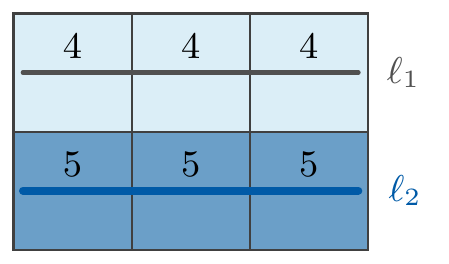
\includegraphics[width=0.76\linewidth]{images/reconstruction_examples/ground_truth_field.png}\\[-0.2ex]
    \small (a) Ground truth and link geometry
  \end{minipage}\hfill
  \begin{minipage}[c]{0.61\textwidth}
    \centering
    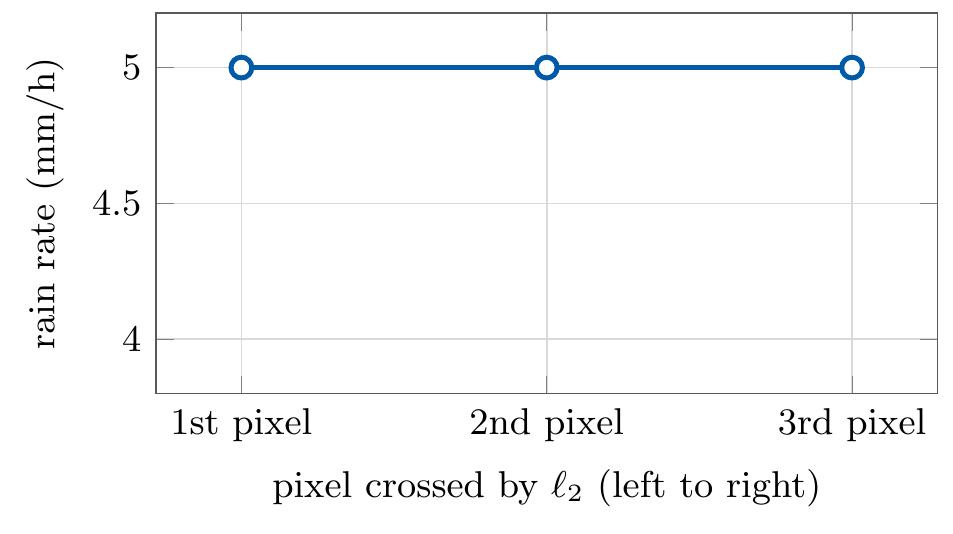
\includegraphics[width=\linewidth]{images/reconstruction_examples/ground_truth_profile_l2.png}\\[-0.2ex]
    \small (b) Ground-truth profile along $\ell_2$
  \end{minipage}

  \vspace{0.7em}

  \begin{minipage}[c]{0.35\textwidth}
    \centering
    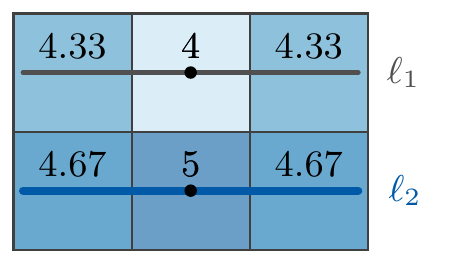
\includegraphics[width=0.76\linewidth]{images/reconstruction_examples/idw_reconstruction_field.png}\\[-0.2ex]
    \small (c) \IDW\ reconstruction
  \end{minipage}\hfill
  \begin{minipage}[c]{0.61\textwidth}
    \centering
    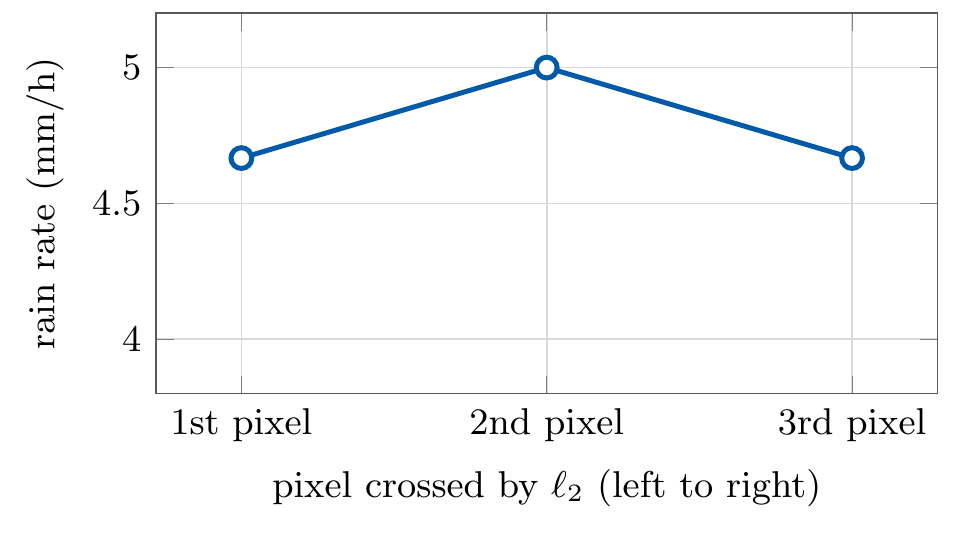
\includegraphics[width=\linewidth]{images/reconstruction_examples/idw_profile_l2.png}\\[-0.2ex]
    \small (d) \IDW\ profile along $\ell_2$
  \end{minipage}

  \vspace{0.7em}

  \begin{minipage}[c]{0.35\textwidth}
    \centering
    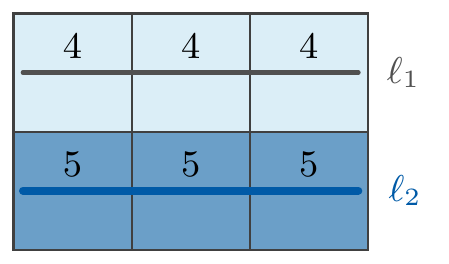
\includegraphics[width=0.76\linewidth]{images/reconstruction_examples/ildw_reconstruction_field.png}\\[-0.2ex]
    \small (e) \ILDW\ reconstruction
  \end{minipage}\hfill
  \begin{minipage}[c]{0.61\textwidth}
    \centering
    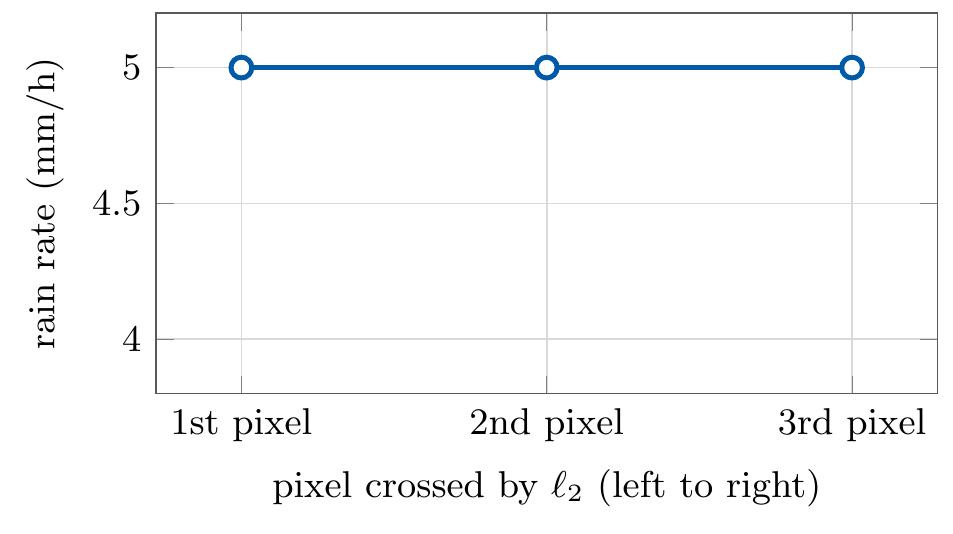
\includegraphics[width=\linewidth]{images/reconstruction_examples/ildw_profile_l2.png}\\[-0.2ex]
    \small (f) \ILDW\ profile along $\ell_2$
  \end{minipage}

  \caption{Geometric difference between midpoint \IDW\ and \ILDW.  Away from
  the middle column, \IDW\ mixes the $5$ \si{\milli\meter\per\hour}
  observation from $\ell_2$ with the neighboring $4$
  \si{\milli\meter\per\hour} observation.  \ILDW\ associates each
  link-level observation with every pixel crossed by its segment and therefore
  exactly recovers this row-wise constant field.}
  \label{fig:idw-ildw-2x3}
\end{figure}

The second link is essential for this normalized-IDW example: if $\ell_2$ were
the only link, its single normalized weight would cancel, and \IDW\ would
return $R_{\ell_2}=5$ at every in-radius pixel.
The \IDW\ underestimation away from the midpoint and the exact \ILDW\ recovery
are illustrated by the six panels in \Cref{fig:idw-ildw-2x3}.

\clearpage
\vspace*{2em}

\subsection{A $3\times3$ Counterexample to Convexity}
\label{appendix:nonconvexity-example}
Consider one horizontal link $\ell$ crossing the three middle-row pixels of a
$3\times3$ grid.  The crossed length is $0.125$~km in each pixel, so
$|\ell|=0.375$~km.  Let the link use horizontal polarization at
$38.003$~GHz, for which the ITU-R coefficients used here are
$\kappa=0.400171594750$ and $\alpha=0.881535333268$.  For this one-link
instance,
\[
\widehat A(R)=\sum_{p\in\ell}d_p\kappa R(p)^\alpha,
\qquad
J_{\mathrm{atten}}(R)=
\frac{\bigl(\widehat A(R)-A_{\mathrm{obs}}\bigr)^2}{|\ell|}.
\]

Take the two strictly positive fields
\[
R^{(L)}=\begin{bmatrix}1&1&1\\20&1&1\\1&1&1\end{bmatrix},
\qquad
R^{(R)}=\begin{bmatrix}1&1&1\\1&1&20\\1&1&1\end{bmatrix}
\quad \si{\milli\meter\per\hour}.
\]
They are left-right reflections across the grid's vertical centerline.  Either
field could be the ground truth: the link crosses the reflected pixels over
equal lengths, so both fields produce
\[
\widehat A\bigl(R^{(L)}\bigr)=\widehat A\bigl(R^{(R)}\bigr)
=A_{\mathrm{obs}}=0.801595407171\ \si{\deci\bel},
\]
and hence
$J_{\mathrm{atten}}(R^{(L)})=J_{\mathrm{atten}}(R^{(R)})=0$.
Their arithmetic mean is
\[
R^{(M)}=\frac{R^{(L)}+R^{(R)}}{2}
=\begin{bmatrix}1&1&1\\10.5&1&10.5\\1&1&1\end{bmatrix}.
\]
For $g(r)=r^\alpha$, we have
$g''(r)=\alpha(\alpha-1)r^{\alpha-2}<0$ because $0<\alpha<1$; hence $g$ is
strictly concave and
$2(10.5)^\alpha>20^\alpha+1$.  Consequently,
\[
\widehat A(R^{(M)})=0.845082934781\ \si{\deci\bel}>A_{\mathrm{obs}},
\qquad
J_{\mathrm{atten}}(R^{(M)})=0.005043106820>0.
\]
Therefore,
\[
J_{\mathrm{atten}}\!\left(\frac{R^{(L)}+R^{(R)}}{2}\right)
>
\frac{J_{\mathrm{atten}}(R^{(L)})+J_{\mathrm{atten}}(R^{(R)})}{2}=0,
\]
which violates the defining inequality for a convex function.  Thus the
physical attenuation term is nonconvex even in this one-link $3\times3$
instance.
% <<<<<<<<<<<<<<<<<<<<<<<<<<<<<<<<<<<<<<<<<<<<<<<<<<<<<<<<<<<<<<<<<<<<<<<
% END ADDITION: APPENDIX ILLUSTRATIVE EXAMPLES
% <<<<<<<<<<<<<<<<<<<<<<<<<<<<<<<<<<<<<<<<<<<<<<<<<<<<<<<<<<<<<<<<<<<<<<<
\end{document}
